%%%%%%%%%%%%%%%%%%%%%%%%%%%%%%%%%%%%%%%%%%%%%%%%%%%%%%%%%%%%%%%%%%%%%
%% This is a (brief) model paper using the achemso class
%% The document class accepts keyval options, which should include
%% the target journal and optionally the manuscript type. 
%%%%%%%%%%%%%%%%%%%%%%%%%%%%%%%%%%%%%%%%%%%%%%%%%%%%%%%%%%%%%%%%%%%%%
\documentclass[journal=jacsat,manuscript=article]{achemso}
%\documentclass[12pt]{article}
%\usepackage[letterpaper,left=0.5in,right=0.5in,top=1.0in,bottom=1.0in]{geometry}

%%%%%%%%%%%%%%%%%%%%%%%%%%%%%%%%%%%%%%%%%%%%%%%%%%%%%%%%%%%%%%%%%%%%%
%% Place any additional packages needed here.  Only include packages
%% which are essential, to avoid problems later. Do NOT use any
%% packages which require e-TeX (for example etoolbox): the e-TeX
%% extensions are not currently available on the ACS conversion
%% servers.
%%%%%%%%%%%%%%%%%%%%%%%%%%%%%%%%%%%%%%%%%%%%%%%%%%%%%%%%%%%%%%%%%%%%%
\usepackage[version=3]{mhchem} % Formula subscripts using \ce{}
\usepackage{siunitx} % generating degrees Celsius in the document 
\usepackage{color}
\usepackage{soul} % allows highlighting text 
\usepackage{makecell}
\usepackage{booktabs}
\usepackage{amsmath}
\usepackage{amssymb}
\usepackage{todonotes}
\usepackage{gensymb}

%%%%%%%%%%%%%%%%%%%%%%%%%%%%%%%%%%%%%%%%%%%%%%%%%%%%%%%%%%%%%%%%%%%%%
%% If issues arise when submitting your manuscript, you may want to
%% un-comment the next line.  This provides information on the
%% version of every file you have used.
%%%%%%%%%%%%%%%%%%%%%%%%%%%%%%%%%%%%%%%%%%%%%%%%%%%%%%%%%%%%%%%%%%%%%
%%\listfiles

%%%%%%%%%%%%%%%%%%%%%%%%%%%%%%%%%%%%%%%%%%%%%%%%%%%%%%%%%%%%%%%%%%%%%
%% Place any additional macros here.  Please use \newcommand* where
%% possible, and avoid layout-changing macros (which are not used
%% when typesetting).
%%%%%%%%%%%%%%%%%%%%%%%%%%%%%%%%%%%%%%%%%%%%%%%%%%%%%%%%%%%%%%%%%%%%%
\newcommand*\mycommand[1]{\texttt{\emph{#1}}}
\DeclareRobustCommand
  \Compactcdots{\mathinner{\cdotp\mkern-2mu\cdotp\mkern-2mu\cdotp}}

%%%%%%%%%%%%%%%%%%%%%%%%%%%%%%%%%%%%%%%%%%%%%%%%%%%%%%%%%%%%%%%%%%%%%
%% Meta-data block
%% ---------------
%% Each author should be given as a separate \author command.
%%
%% Corresponding authors should have an e-mail given after the author
%% name as an \email command. Phone and fax numbers can be given
%% using \phone and \fax, respectively; this information is optional.
%%
%% The affiliation of authors is given after the authors; each
%% \affiliation command applies to all preceding authors not already
%% assigned an affiliation.
%%
%% The affiliation takes an option argument for the short name.  This
%% will typically be something like "University of Somewhere".
%%
%% The \altaffiliation macro should be used for new address, etc.
%% On the other hand, \alsoaffiliation is used on a per author basis
%% when authors are associated with multiple institutions.
%%%%%%%%%%%%%%%%%%%%%%%%%%%%%%%%%%%%%%%%%%%%%%%%%%%%%%%%%%%%%%%%%%%%%
\author{Stephen P. Vicchio}
\affiliation[Clemson University]
{Department of Chemical and Biomolecular Engineering, Clemson University, Clemson, SC}
\author{Sachi Hilliard}
\affiliation[Clemson University]
{Department of Chemical and Biomolecular Engineering, Clemson University, Clemson, SC}
%\author{Omar Farha?}
%\affiliation[Northwestern University]
%{Northwestern University}
\author{Rachel B. Getman}
\email{rgetman@g.clemson.edu}
\affiliation[Clemson University]
{Department of Chemical and Biomolecular Engineering, Clemson University, Clemson, SC}


%%%%%%%%%%%%%%%%%%%%%%%%%%%%%%%%%%%%%%%%%%%%%%%%%%%%%%%%%%%%%%%%%%%%%
%% The document title should be given as usual. Some journals require
%% a running title from the author: this should be supplied as an
%% optional argument to \title.
%%%%%%%%%%%%%%%%%%%%%%%%%%%%%%%%%%%%%%%%%%%%%%%%%%%%%%%%%%%%%%%%%%%%%
\title[manuscript]{Nickel(II) and Copper(II) Supported Metal Complex Stability in NU-1000 Under Hydrogenation Conditions}

%%%%%%%%%%%%%%%%%%%%%%%%%%%%%%%%%%%%%%%%%%%%%%%%%%%%%%%%%%%%%%%%%%%%%
%% Some journals require a list of abbreviations or keywords to be
%% supplied. These should be set up here, and will be printed after
%% the title and author information, if needed.
%%%%%%%%%%%%%%%%%%%%%%%%%%%%%%%%%%%%%%%%%%%%%%%%%%%%%%%%%%%%%%%%%%%%%
\abbreviations{IR,NMR,UV}
\keywords{American Chemical Society, \LaTeX}

%%%%%%%%%%%%%%%%%%%%%%%%%%%%%%%%%%%%%%%%%%%%%%%%%%%%%%%%%%%%%%%%%%%%%
%% The manuscript does not need to include \maketitle, which is
%% executed automatically.
%%%%%%%%%%%%%%%%%%%%%%%%%%%%%%%%%%%%%%%%%%%%%%%%%%%%%%%%%%%%%%%%%%%%%
\begin{document}

%%%%%%%%%%%%%%%%%%%%%%%%%%%%%%%%%%%%%%%%%%%%%%%%%%%%%%%%%%%%%%%%%%%%%
%% The "tocentry" environment can be used to create an entry for the
%% graphical table of contents. It is given here as some journals
%% require that it is printed as part of the abstract page. It will
%% be automatically moved as appropriate.
%%%%%%%%%%%%%%%%%%%%%%%%%%%%%%%%%%%%%%%%%%%%%%%%%%%%%%%%%%%%%%%%%%%%%
%\begin{tocentry}
%
%Some journals require a graphical entry for the Table of Contents.
%This should be laid out ``print ready'' so that the sizing of the
%text is correct.
%
%Inside the \texttt{tocentry} environment, the font used is %Helvetica
%8\,pt, as required by \emph{Journal of the American Chemical
%Society}.
%
%The surrounding frame is 9\,cm by 3.5\,cm, which is the maximum
%permitted for  \emph{Journal of the American Chemical Society}
%graphical table of content entries. The box will not resize if the
%content is too big: instead it will overflow the edge of the box.
%
%This box and the associated title will always be printed on a
%separate page at the end of the document.
%
%\end{tocentry}

%%%%%%%%%%%%%%%%%%%%%%%%%%%%%%%%%%%%%%%%%%%%%%%%%%%%%%%%%%%%%%%%%%%%%
%% The abstract environment will automatically gobble the contents
%% if an abstract is not used by the target journal.
%%%%%%%%%%%%%%%%%%%%%%%%%%%%%%%%%%%%%%%%%%%%%%%%%%%%%%%%%%%%%%%%%%%%%
\begin{abstract}
    
\end{abstract}

%%%%%%%%%%%%%%%%%%%%%%%%%%%%%%%%%%%%%%%%%%%%%%%%%%%%%%%%%%%%%%%%%%%%%
%% Start the main part of the manuscript here.
%%%%%%%%%%%%%%%%%%%%%%%%%%%%%%%%%%%%%%%%%%%%%%%%%%%%%%%%%%%%%%%%%%%%%
\newpage
\section{Introduction}

%\begin{figure}[t]
%    \centering
%    \includegraphics[width=0.95\textwidth]{zi-images/00-General-Graphics/2020-07-31-Combined-%MOF-Figure-final.png}
%    \caption{The structure of NU-1000, which is comprised of (a)  inorganic nodes %(\ce{[Zr6(\mu3-O)4(\mu3-OH)4(H2O)4(OH)4]^8^+}) and (b) organic linkers %(1,3,6,8-tetrakis(p-benzoic acid)pyrene (\ce{TBAPy^4^-})) to produce (c) the framework %structure (with the c-pore highlighted by the gray box). Additionally, the two metal %complexes supported in the c-pore of NU-1000 are also shown: (d) the \ce{Cu3(OH)4} metal %complex, and (d) the 1-\ce{Ni4(OH)6} (purple) metal complex.}
%    \label{fig:MOFstructure}
%\end{figure}

% Paragraph 1: Knowledge gap related to the problem about knowing the precise structure of the active site (both when synthesized and then when activated)
\subsection{Paragraph 0}
 Catalysts are vital to the present and future of society, with currently 90\% of the world's consumer goods requiring a catalyst during manufacturing.\cite{Hagen2015} Most industrially relevant catalysts are heterogeneous because of their robustness to reaction conditions and ease of recovery. However, standard bulk heterogeneous catalysts suffer from poorly defined active sites that inhibit molecular understandings of the precise catalyst structure and catalytic mechanisms; this lack of knowledge has limited rational catalyst design for bulk metal catalysts. Over the last two decades, a new area of heterogeneous catalysis has emerged involving metal-organic frameworks (MOFs). MOFs, a porous material formed from inorganic nodes interconnected by organic linkers, function as both a heterogeneous catalysts and catalyst supports.\hl{REFERENCE} MOFs exhibit a diverse platform of tunable structures with well-defined active sites and chemical functionality thus making them an attractive material for single-atom catalysis. 
 % note to self.. I think the end of this paragraph is OKAY.. it's the beginning that needs work.

% There's the large review paper that is good for the introduction section. --> WHICH IS WHAT, STEPHEN? Be sure to write down the review paper...  

\subsection{Paragraph 1}
Within the scientific community, the \ce{Zr} based MOF NU-1000 is commonly used as a catalyst support for 3d metal complexes. Structurally, the NU-1000 MOF contains \ce{Zr} nodes interconnected by carbon based pyrene linkers to generate both large hexagonal channels (30 A), triangular channels (10 A), and small pores (8 A).(\hl{REFERENCE}) The staggered arrangement of protons forming \ce{OH}- and \ce{OH2}-ligand pairs on the node generate anchoring sites for 3d transition metals.\cite{Planas2014} Deposition of 3d transition metal atoms on the MOF framework occurs in the vapor phase via atomic layer deposition (ALD) in MOFs (AIM) \hl{REFERENCE} and in condensed phase via solvothermal deposition in MOFs (SIM) \hl{REFERENCE}. The \ce{OH_{x}}-ligands within the small pore (\~8 A) of NU-1000 preferentially bind the metal species within the framework,\cite{Gallington2016,Rimoldi2017} and the synthesis conditions regulate the active species loading to generate complex active site structures.\cite{Kim2015} Elucidating the exact structure of the active site is challenging; characterization of the metal active sites is suppressed by the bulk framework structure, leading to questions about the structure and composition of the synthesized active site.

% Paragraph 2: More specific issue and problems 
% the different types of potential models for these systems.. there are different modeling choices that can be made for these systems.. talk about the different Ni(II) models comprised of a single Ni(II) atoms.. 
\subsection{Paragraph 2}
Combined experimental characterization and computational modeling has provided insights the active site structure for 3d transition metals supported on the standard NU-1000 MOF framework. The primary focus remains understanding the exact composition of the active site structure that are dependent on the number of metal species. A mononuclear (single-site) model was originally thought to be the active site structure for metals supported on NU-1000.\cite{Li2016sintering,AbdelMageed2019,Gallington2016} Mechanistic investigations into ethylene hydrogenation\cite{Shabbir2020} and propyne partial hydrogenation and isomerization\cite{Hackler2020} use a mononuclear model to high-throughout screen different metal species. \citeauthor{Shabbir2020} demonstrates the different proton tolopogies the mononuclear active site can adopt,\cite{Shabbir2020} while \citeauthor{Hackler2020} investigates two different \ce{H2} splitting pathways on a mononuclear active site.\cite{Hackler2020} A potential limitation of these findings, however, is the usage of a mononuclear model. The structure of the active site has been refined revealing that the metal species supported in the c-pore are more likely to be multinuclear (i.e., consisting of multiple metal species). Using difference envelope density (DED),\cite{Li2017} and differential pair distribution function (dPDF) analysis,\cite{PlateroPrats2017} the formation of multinuclear clusters within the c-pore has been established as the active site for NU-1000. A recent study by \citeauthor{Kim2020}  illustrates the multinuclearity of the active site by determining metal loading per node for different metal precursors.\cite{Kim2020} With metal complex deposition occurring only within the c-pore using the ALD process, metal loading greater than 2 metal atoms per node suggest an active site containing multiple metal atoms. Providing further insight to the multinuclear active site structure for \ce{Ni} complexes, \citeauthor{PlateroPrats2017} suggest the formation of tetranuclear heterobimetallic nanowires spanning the length of the c-pore with the cluster attached to two nodes.\citeauthor{PlateroPrats2017} For \ce{Cu} complexes, \citeauthor{Ikuno2017} proposes a similar trinuclear structure that also spans the c-pore of NU-1000. Experimentally, the nature of the active site for metal complexes on NU-1000 is multinuclear rather than mononuclear; however, the precise structure of the multinuclear active site remains unknown. 

\subsection{Paragraph 3}
Further complicating our understanding of the active site structure is the structural changes induced  by the reaction environment during both the activation step and the reaction steps. The activation environment, and therefore the structural changes, determine the reaction mechanism, such as dehydrogenation, hydrogenation, dimerization, oligomerization. The reaction environment includes both the temperature and gas phase species. \citeauthor{Kim2015} experimentally determined that the metal loading of \ce{In} deceased from  6 \ce{In} per node to 2 \ce{In} per node as the temperature increased from \SI{80}{Celsius} to \SI{200}{Celsius}.\cite{Kim2015} For ethylene hydrogenation, \citeauthor{Li2016sintering} proposes a mechanism on a mononuclear (single-site) \ce{Ni(II)} complex that is activated with \ce{H2} gas to form a \ce{Ni} hydride by removing a coordinated \ce{OH}-ligand.\cite{Li2016sintering} In a similar \ce{H2} environment, \citeauthor{Halder2020} experimentally demonstrated that above \SI{200}{Celsius} the trinuclear \ce{Cu(II)}-clusters supported on NU-1000 are reduced to zero-valent \ce{Cu(0)} species and stripped away from the node with the NU-1000 framework reverting back to the original unit cell dimensions.\cite{Halder2020} Conversely, when exposed to similar reducing conditions the tetranuclear \ce{Ni(II)} cluster shows only subtle structural variations up to 200 oC\cite{PlateroPrats2017} suggesting the cluster is stable under these conditions and that the initial activation only produces subtle changes into the structure of the cluster. Proposed dimerization mechanisms on the tetranuclear \ce{Ni(II)} cluster activate with \ce{Et2AlCl} to remove \ce{OH}-ligands within the cluster as coordinated \ce{H2O} species and generate the active \ce{C2H5}$^*$ species coordinated to the \ce{Ni} atoms.\cite{Ye2017} Using a mononuclar site \ce{Co} cluster, \citeauthor{Li2017} proposes an activation step involving \ce{O2} gas that removes a coordinated \ce{H2O} and alters the coordination environment of the \ce{Co} atom. The metal complexes supported on MOFs, here specifically NU-1000, demonstrate structural variations depending on reaction conditions. To further our understanding of these metal complex active site structures and design better catalysts, there is a need to understand the transformation of the active site structure depending on the reaction environment. 

\subsection{Paragraph 4}
Herein our work addresses questions related to the structural changes of the metal complex active site as a function of both temperature and gas phase conditions. By combining Density Functional Theory (DFT) calculations with gas phase empirical models, we investigate cluster stability under different gas phase conditions (\ce{H2}) and temperature. Modeling focuses on the 1-\ce{Ni4(OH)6} (purple) cluster proposed by \citeauthor{PlateroPrats2017} and the \ce{Cu3(OH)4} cluster proposed by \cite{Ikuno2017}. Our results provide structural information about the types of changes exhibited by the cluster to establish more appropriate molecular models. 

\newpage
%%%%%%%%%%%%%%%%%%%%%%%%%%%%%%%%%%%%%%%%%%%%%%%%%%%%%%%%%%%%%%%%%%%%%
%% Methodology
%%%%%%%%%%%%%%%%%%%%%%%%%%%%%%%%%%%%%%%%%%%%%%%%%%%%%%%%%%%%%%%%%%%%%

\section{Methodology}
We investigate how reaction conditions, such as temperature ($T$) and pressure ($P$), influence the structure and composition of a \ce{Ni(II)} supported metal complex on NU-1000. Figure \ref{fig:Ni-MOF-model} shows the NU-1000 MOF and the location of the \ce{Ni(II)} supported metal complex within the small pore of NU-1000 (pore diameter of 8 {\AA}). The proposed model consists of four \ce{Ni(II)} species located within the small-pore as shown in Figure 1 (d) and (e).\cite{PlateroPrats2017,Ye2017} Structurally, the \ce{Ni(II)} atoms are linked together by \ce{\mu3-OH} and \ce{\mu2-OH} ligands that connect adjacent \ce{Zr} nodes of the small-pore. Depending on conditions, the \ce{Ni} atoms may also be coordinated with adsorbed \ce{H2O} species as shown in Figure \ref{fig:Ni-MOF-model} (d) and (e). 

\begin{figure}[H]
    \centering
    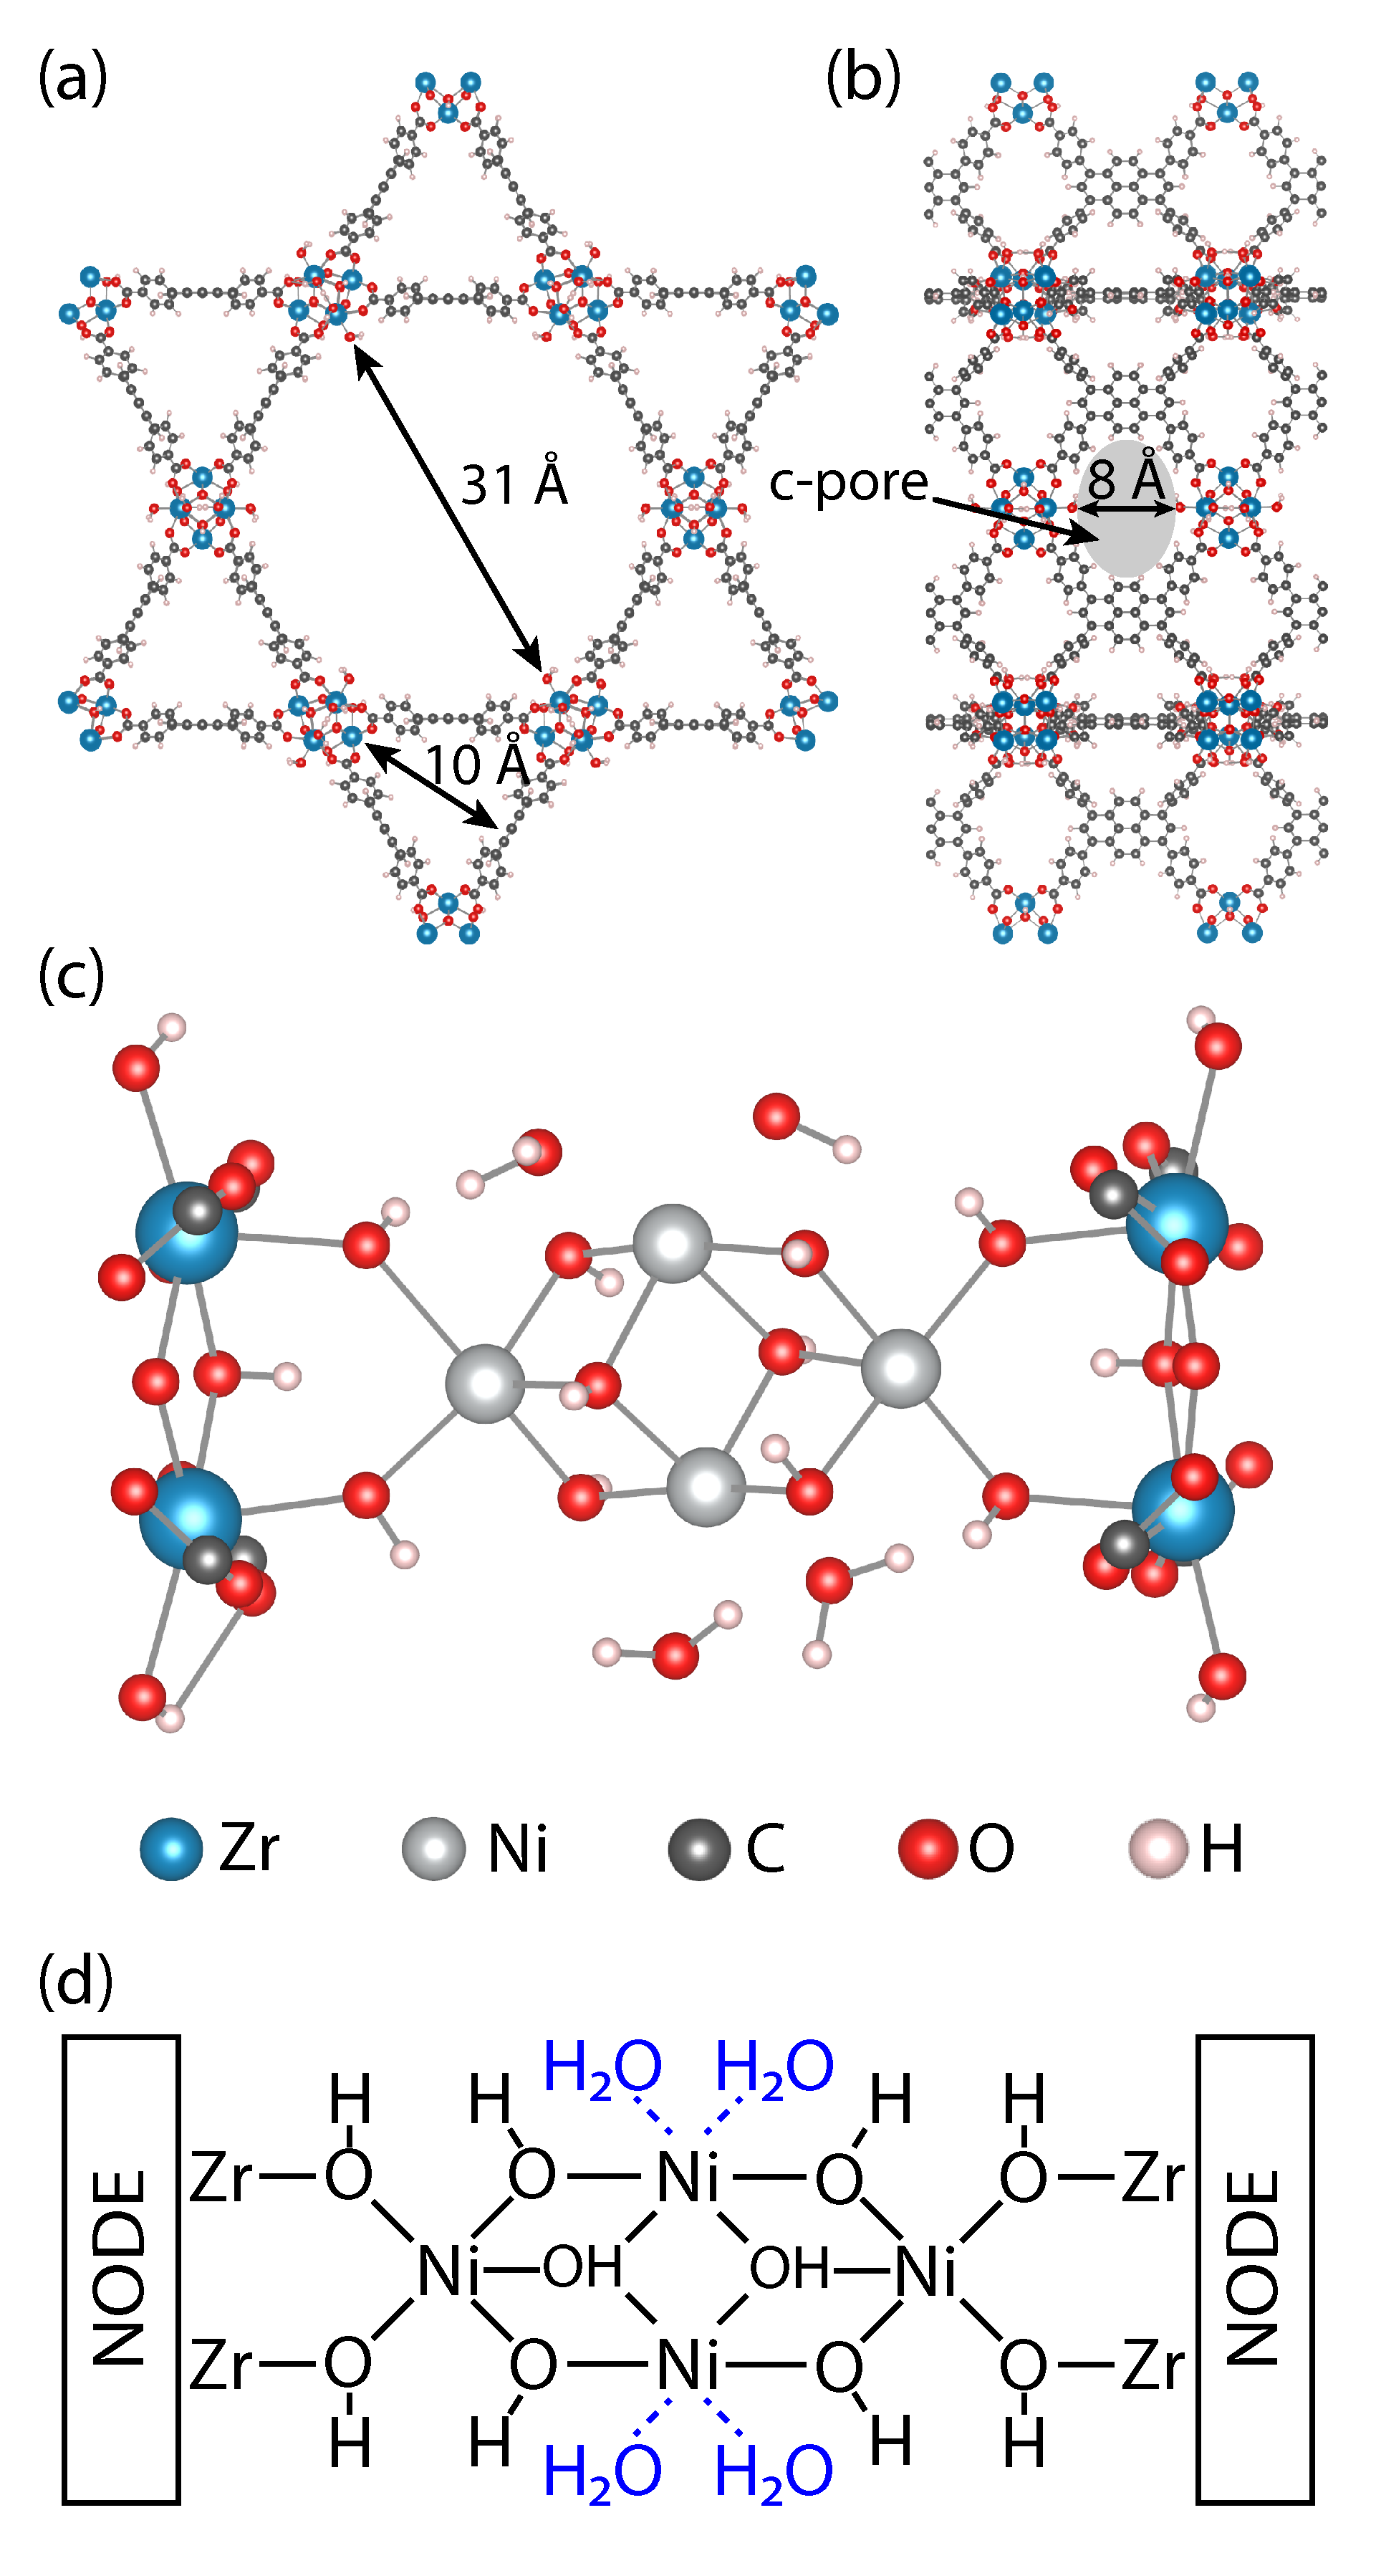
\includegraphics{zi-images/00-General-Graphics/2021-figure-MOF-structure.png}
    \caption{
    The structure of NU-1000 shown along the (a) c-axis and the (b) a-axis with the location of the metal complex location highlighted by the gray box. The proposed structure for the tetranuclear \ce{Ni} cluster is shown (c) atomistically and (d) schematically, with the MOF framework truncated from the renderings.}
    \label{fig:Ni-MOF-model}
\end{figure}

We select the \ce{Ni4(OH)6.4H2O} model, shown in Figure \ref{fig:Ni-MOF-model} \hl{(d) and (e)}, to be the as-synthesized \ce{Ni} structure and the reference structure for our investigation. While investigating how reaction conditions alter the catalyst structure, all structural and compositional transformations start from the \ce{Ni4(OH)6.4H2O} model, that is we explore the evolution of the composition and structure starting from the \ce{Ni4(OH)6.4H2O} model. Under \ce{H2}, both the \ce{Ni(II)} and \ce{OH} ligands provide sites that can accept dissociated \ce{H} atoms after \ce{H2} adsorption and dissociation. When these sites, defined as \ce{OH^{*}} and \ce{Ni^{*}}, accept dissociated \ce{H} atoms, the composition of the cluster changes to include additional adsorbed \ce{H2O} (\ce{H2O^{*}}) and/or Nickel-hydride (\ce{Ni-H}). However, the adsorbed \ce{H2O} are not fixed to the \ce{Ni} cluster; our modeling includes the subsequent desorption of \ce{H2O} into the gas-phase. All the aforementioned transformations are dependent on the reaction temperature ($T$), and \ce{H2} ($P_{\text{\ce{H2}}}$) and \ce{H2O} ($P_{\text{\ce{H2O}}}$) partial pressures. We model how the cluster structure and composition changes as a function of these different conditions by computing the free energy of compositionally different model structures  relative to a reference structure. We consider the chemical transformed described by the reversible reaction shown below (Equation \ref{eq:chemical-formula}):
\begin{equation}
    \begin{split}
        \ce{Ni4(OH)6.4H2O + xH2 (g) <=> Ni4(OH)_{10-(y+z)}(H)_{4+2x-(x+y)}.yH2O + zH2O (g)} \\
    \end{split}
    \label{eq:chemical-formula}
\end{equation}
where x defines the \ce{H2} added to the cluster, y is the number of adsorbed \ce{H2O} on the \ce{Ni} cluster, and z is the number of \ce{H2O} in the gas phase. We look at the thermodynamic stability of different modified clusters (\ce{Ni4(OH)_{10-(y+z)}(H)_{4+2x-(x+y)}}) that contain varying compositions of adsorbed (y) and gaseous (z) \ce{H2O} relative to the \ce{Ni4(OH)6.4H2O} model cluster. 

We generate a library of unique, modified structures by systematically adding \ce{H} atoms to the \ce{Ni^{*}} and \ce{OH^{*}} sites on the metal cluster. The \ce{H} addition process creates a new structure that is structurally and compositionally different from the reference structure. The new structure contains either \ce{Ni-H} or \ce{H2O^{*}}. The adsorbed \ce{H2O^{*}} is systematically removed thereby creating new structures. For these new structures, we again add \ce{H} atoms to the \ce{Ni^{*}} and \ce{OH^{*}} sites on the metal cluster and repeat the removal of any adsorbed \ce{H2O}. The iterative process creates a library of structures that are structurally and compositionally unique with \ce{H^{*}}, \ce{OH^{*}}, and \ce{Ni^{*}}. 

To determine the stability of the different structural and compositional variations for the \ce{Ni} metal complex, we calculate the relative free energy referenced to the \ce{Ni4(OH)6.4H2O} for each structure in library using \textit{ab initio} thermodynamic analysis. The approach requires a transformation of the free energy from a fixed number of atoms ($N_{\text{i}}$) to a fixed chemical potential ($\mu_{\text{i}}$). The free energy is transformed with respect to $\mu_{\text{H}^{*}}$, $\mu_{\text{OH}^{*}}$, and $\mu_{\text{Ni}^{*}}$ to account for structural and compositional variations in the number of adsorbed \ce{H} species ($N_{\text{H}^{*}}$), \ce{OH}-ligands ($N_{\text{OH}^{*}}$), and \ce{Ni} species ($N_{\text{Ni}^{*}}$). Equation \ref{eq:free-energy-trans} shows the free energy difference ($\Delta F^{(3)}(T,\mu_{\text{H}^{*}},\mu_{\text{OH}^{*}},\mu_{\text{Ni}^{*}})$) between structure $\text{j}$ and the \ce{Ni4(OH)6} reference structure (ref).
\begin{equation}
    \begin{split}
        \Delta F^{(3)}(T,\mu_{\text{H}^{*}},\mu_{\text{OH}^{*}},\mu_{\text{Ni}^{*}})  
        & = \Delta F^{(0)} - (\mu_{\text{H}^{*}})(\Delta N_{\text{H}^{*}}) \\ 
        & - (\mu_{\text{OH}^{*}})(\Delta N_{\text{OH}^{*}}) - (\mu_{\text{Ni}^{*}})(\Delta N_{\text{Ni}^{*}}) \\ 
    \end{split}
    \label{eq:free-energy-trans}
\end{equation}
The $\Delta F^{(0)}$ is the untransformed free energy difference between structure $\text{j}$ ($F_{\text{j}}$) and the reference structure ($F_{\text{ref}}$). The $F_{\text{j}}(T,N_{\text{j},\text{H}^{*}},N_{\text{j},\text{OH}^{*}},N_{\text{j},\text{Ni}^{*}})$ term is the free energy of structure $\text{j}$ with configuration of $N_{\text{j},\text{H}^{*}}$, $N_{\text{j},\text{OH}^{*}}$, and $N_{\text{j},\text{Ni}^{*}}$. We approximate the free energy ($F_{\text{j}}$) using the electronic energy from density functional theory (DFT). The $\Delta N$ terms are the difference between $N_{\text{j}}$ and $N_{\text{ref}}$ for each transformed species.

%We assume that $\ce{\text{H}^{*}}$ and $\ce{\text{OH}^{*}}$ are in equilibrium with an ideal-gas like reservoir with of %\ce{H2} and \ce{H2O}, respectively (as shown in Figure \ref{fig:FPT-process}). The chemical potential of the reservoir is %dependent on the reaction conditions ($T$ and $P$). The assumed equilibrium for $\ce{\text{H}^{*}}$ is with $\frac{1}{2}$ %\ce{H2} (g) and for $\ce{\text{OH}^{*}}$ is with \ce{H2O} (g)/$\frac{1}{2}$\ce{H2} (g) (Equation %\ref{eq:reaction_equilibrium}). The combined expression for $\ce{OH^{*}}$ captures the influence of both \ce{H2O} and %\ce{H2} gas phase conditions on the stability of the cluster (further details in the Supporting Information).
%\begin{equation}
%    \begin{split}
%        \frac{1}{2} H_{2} (g) & \ce{<=>} H^{*} \\           
%        \frac{1}{2} H_{2} (g) + OH^{*} & \ce{<=>} H_{2}O (g)  
%    \end{split}
%    \label{eq:reaction_equilibrium}
%\end{equation}
%Using Equation \ref{eq:reaction_equilibrium}, the relationship between the $\ce{\text{H}^{*}}$ and $\ce{OH^{*}}$ species %and the gas phase \ce{H2} and \ce{H2O} conditions are shown in Equation \ref{eq:chemicalpotentialeq}. The %$\mu_{i}^{g}(T,P)$ terms contain the temperature and pressure influences of the reaction conditions. 
%\begin{equation}
%    \begin{split}
%        \mu_{H^{*}} &= \frac{1}{2} \mu_{H_{2}}^{g}(T,P) \\ 
%        \mu_{OH^{*}} &= \mu_{H_{2}O}^{g}(T,P) - \frac{1}{2} \mu_{H_{2}}^{g}(T,P) \\
%    \end{split}
%    \label{eq:chemicalpotentialeq}
%\end{equation}

The chemical potential terms, $\mu_{\text{H}^{*}}$ and $\mu_{\text{OH}^{*}}$, include the temperature and pressure dependencies.\cite{Reuter2003,Reuter2004,Grundner2015,Paolucci2016,Li2016,Getman2008,Mandal2020}. We relate $\mu_{\text{H}^{*}}$ and $\mu_{\text{OH}^{*}}$ to $\mu_{\text{\ce{H2}}}^{\text{g}}(T,P)$ and $\mu_{\text{\ce{H2O}}}^{\text{g}}(T,P)$ by assuming each species is in equilibrium with an ideal gas-reservoir. The gas phase chemical potential terms, $\mu_{i}^{g}(T,P)$, are computed by correcting the electronic energy (referenced at $T$=0 K) of an isolated molecule with a chemical potential term, $\Delta \mu_{H_{2}}(T,P)$, that includes all the temperature- and pressure- dependent free-energy contributions (Equation \ref{eq:chemicalpotentialrel} ).
\begin{equation}
    \begin{split}
    \mu_{\text{i}}^{\text{g}}(T,P) &= E_{\text{i}} + \Delta \mu_{\text{i}}(T,P)  \\  
    \mu_{\text{i}}^{\text{g}}(T,P) &= E_{\text{i}} + \Big[ \Delta G_{\text{i}}(T,P^{o}) + RT \ln{\Big( \frac{P_{\text{i}}}{P^{o}} \Big)} \Big]  \\ 
    \end{split}
    \label{eq:chemicalpotentialrel}
\end{equation}
where $\text{i}$ represents either species \ce{H2} or \ce{H2O}. The gas-phase Gibbs free energies ($\Delta G_{\text{i}}(T,P^{o})$) at standard pressure ($P^{o}$) were computed using the NASA Polynomials\cite{Mcbride1993} in the pMuTT\cite{LYM2019106864} Python package. For \ce{Ni}, we approximate the chemical potential term ($\mu_{\text{Ni}^{*}}$) using the electronic energy of a bulk \ce{Ni} metal system. \hl{XXXX of the Supporting Information contains the full derivation for the \textit{ab initio} thermodynamic modeling approach.} 

We calculate $\mu_{\text{i}}^{\text{g}}(T,P)$ for both \ce{H2} and \ce{H2O} at temperatures ranging from 20 \degree C to 320 \degree C and \ce{H2} partial pressure ranging from $10^{-30}$ bar to $10^{5}$ bar at a fixed \ce{H2O} partial pressure of $10^{-9}$ bar. For each structure in the library, the free energy (Equation \ref{eq:free-energy-trans}) is calculated under range of activation conditions. For a given set of reaction conditions, we determined the most thermodynamically favorable structure by determining which structure minimizes the free energy (Equation \ref{eq:free-energy-trans}).  

The energies for the structures are from periodic density functional (DFT) calculations in CP2K.\cite{Hutter2014} The exchange correlation energy was calculated with the PBE functional\cite{Perdew1996} and corrected using damped D3 dispersion corrections formulated by \citeauthor{Grimme2010}.\cite{Grimme2010} The DZVP-MOLOPT basis set describes the valance electrons, Goedecker pseudopotentials\cite{Goedecker1996} describes the core electrons. The plane wave cutoff energy is 360 Ry and  all atoms in the periodic unit cell were allowed to relax during geometry optimizations (see Supporting information for a sample input file for further computational details). The variable spin states of the metal atoms required Unrestricted Kohn-Sham (UKS). For example, \ce{Ni(II)} can adopt both singlet (no unpaired electrons) and triplet (two unpaired electron) configurations. For clusters consisting of multiple \ce{Ni} atoms, we consider spin state permutations within the library of model structures. Any structures exhibiting spin contamination were removed from the analysis (see support information for more details).

\hl{How the PDFs are calculated from the model structures is something that is going to need to be included by Karena and Woodrow here.}

%%%%%%%%%%%%%%%%%%%%%%%%%%%%%%%%%%%%%%%%%%%%%%%%%%%%%%%%%%%%%%%%%%%%%
%% Results
%%%%%%%%%%%%%%%%%%%%%%%%%%%%%%%%%%%%%%%%%%%%%%%%%%%%%%%%%%%%%%%%%%%%%
\newpage
\section{New Results}


\section{Old Results}
We create phase diagrams that show the stability of different configurations and clusters as a function of $T$, $P_{\text{\ce{H2}}}$, and $P_{\text{\ce{H2O}}}$. At each set of conditions, the structure with the lowest free energy is identified and plotted to produce the phase diagram. The regions on the phase diagram correspond to a specific low energy structure, and at the interface between two regions the free energies values are the same. The phase diagrams show structural stability at a fixed \ce{H2O} partial pressure, which allows us to generate phase diagrams only as a function of $T$ and $P_{\text{\ce{H2}}}$. Experimentally, the conditions the tetranuclear \ce{Ni(II)} cluster is exposed to do not contain any \ce{H2O} gas; therefore, we assume a small value for \ce{H2O} partial pressure ($P_{\text{\ce{H2O}}}$) of $10^{-9}$ bar. We provide a phase diagram describing the \ce{H2O} evolution from a \ce{Ni4(OH)6.4H2O} model as a function of $T$ and $P_{\text{\ce{H2O}}}$ in the \hl{Supporting Information}.

\todo[inline]{Update the figure below.}
\begin{figure}[H]
    \centering
    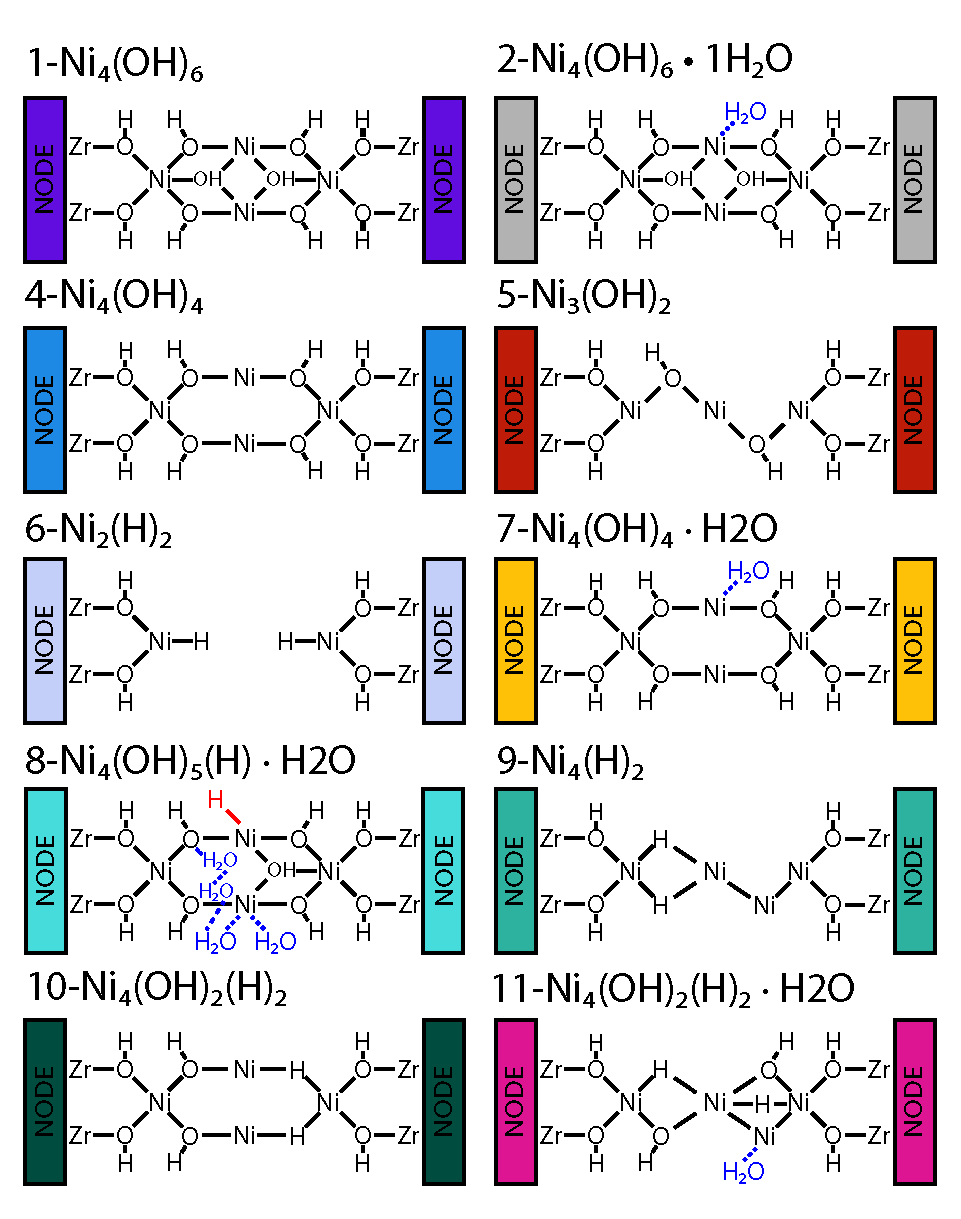
\includegraphics{zi-images/01-Ni-Graphics/2021-figure-structure-Ni-transformations_manuscript-structure.png}
    \caption{
    Schematic representation of the structures that minimize the free energy expression (\ref{eq:free-energy-trans}) the \textit{ab initio} thermodynamic analysis. The blue colored \ce{H2O}s indicate \ce{H2O} coordinated to \ce{Ni} atoms and the red colored \ce{H} atoms indicate the formation of a \ce{Ni-H}.
    \hl{This figure will ALSO need to be updated.. show only the structures that are absolutely necessary here now.}} 
    \label{fig:Ni-structure-diagram}
\end{figure}

Under the studied reaction conditions, the stable structures that minimize the free energy during \textit{ab initio} thermodynamic analysis are shown in Figure \ref{fig:Ni-structure-diagram}. Figure \ref{fig:Ni-structure-diagram} demonstrates the diverse structural landscape of the \ce{Ni4} metal complex. For example, model 2-\ce{Ni4(OH)6.H2O} (gray) contains adsorbed \ce{H2O} coordinated to one of the \ce{Ni} atoms and model 8-\ce{Ni4(OH)5(H).4H2O} (teal) contains a \ce{Ni-H} species. Additionally, we observe structures containing the loss of \ce{Ni} atoms (model 6-\ce{Ni2(H)2} (lilac)). The phase diagram describing the different conditions for these structures is shown in Figure \ref{fig:phase_diagram_Ni_combined}. 

% fully transforming Phase diagram 
\begin{figure}[H]
    \centering
    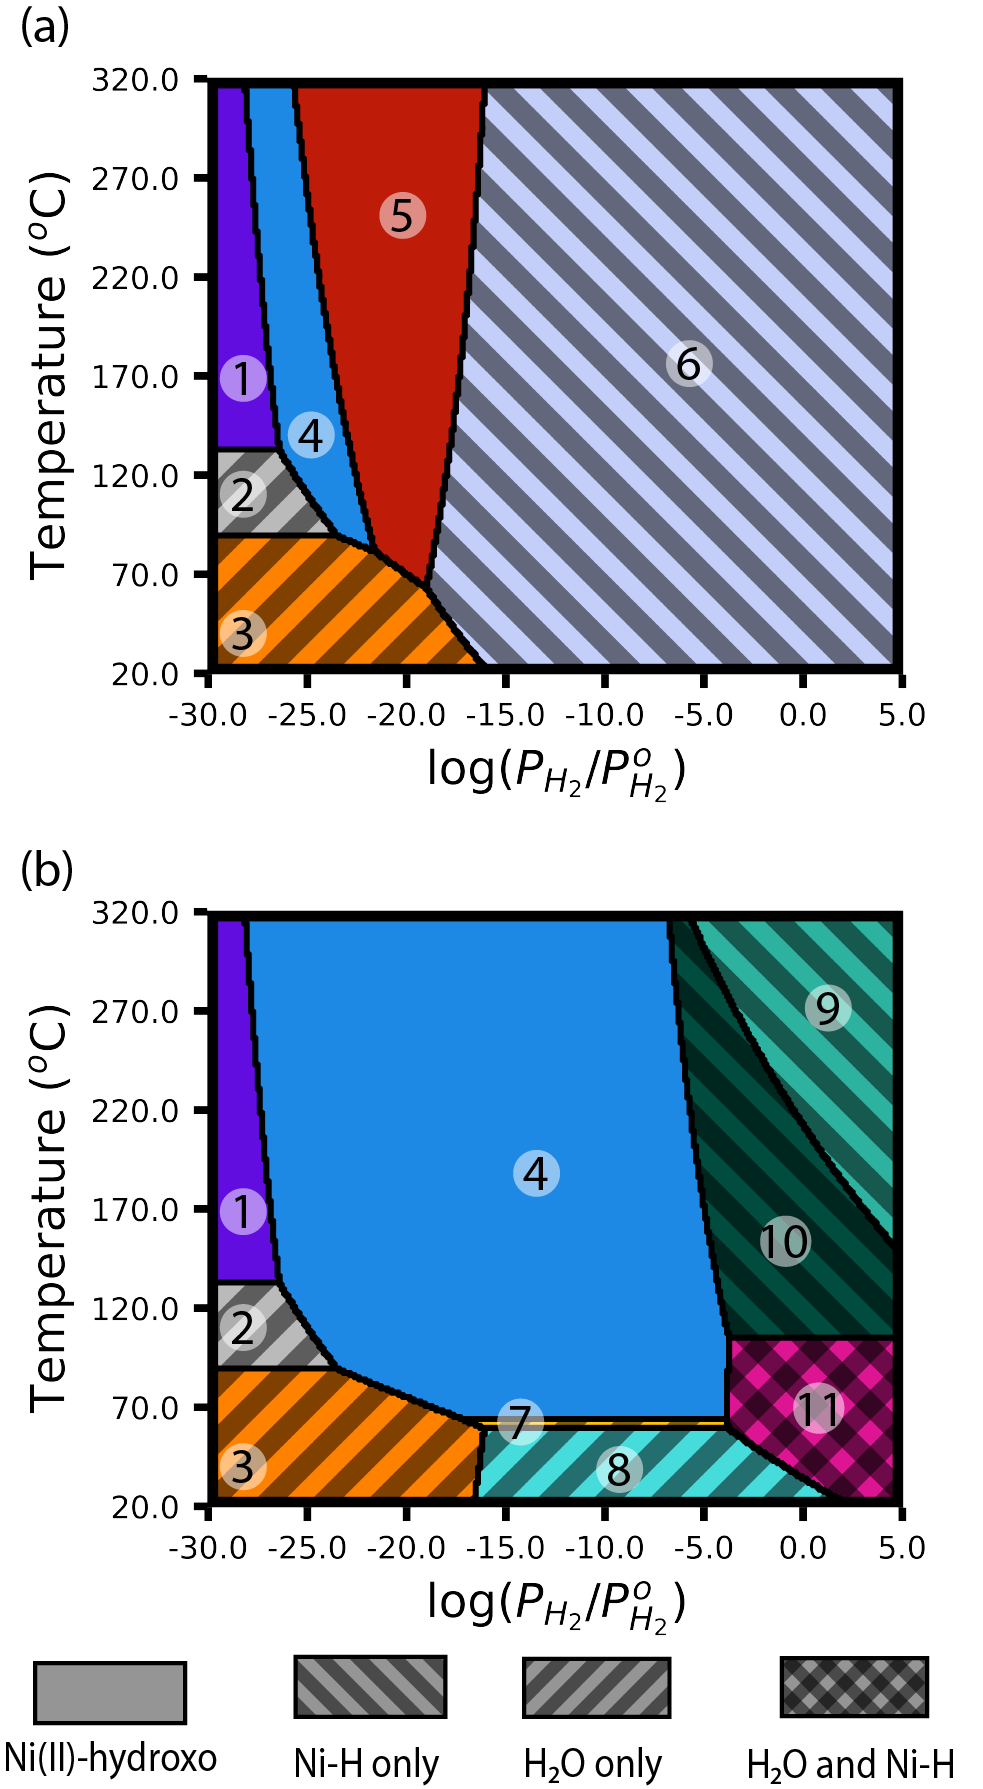
\includegraphics{zi-images/01-Ni-Graphics/2021-03-23-Ni-phase-diagram-combined-manuscript.png}
    \caption{
    The stability of the \ce{Ni(II)} cluster as a function of temperature and \ce{H2} partial pressure at a \ce{H2O} partial pressure = $10^{-9}$ bar when transforming with (a) \ce{H^{*}}, \ce{OH^{*}}, and \ce{Ni^{*}} and, (b) \ce{H^{*}} and \ce{OH^{*}} (fixed \ce{Ni^{*}}). \hl{Regions indicate the the modified structure that minimizes the free energy} Equation (\ref{eq:free-energy-trans}) at a given combination of $T/P_{H_{2}}$ and fixed \ce{H2O} partial pressure. The \ce{H2} partial pressure is reported as $log(P_{H_{2}}/P_{H_{2}}^{o})$, where the standard state is 1 bar. The following naming convention is adopted for the structures: 
    1-\ce{Ni4(OH)6} (purple),              % purple
    2-\ce{Ni4(OH)6.H2O} (gray),            % gray
    3-\ce{Ni4(OH)6.4H2O} (orange),         % orange
    4-\ce{Ni4(OH)4} (light blue),          % light blue
    5-\ce{Ni3(OH)2} (red),                 % red
    6-\ce{Ni2(H)2} (lilac),                % lilac 
    7-\ce{Ni4(OH)4.H2O} (yellow),         % yellow
    8-\ce{Ni4(OH)5(H).4H2O} (teal),        % teal 
    9-\ce{Ni4(H)2} (mint),                 % mint 
    10-\ce{Ni4(OH)2(H)2} (green), and      % green 
    11-\ce{Ni4(OH)2(H)2.H2O} (pink).       % pink 
    }
    \label{fig:phase_diagram_Ni_combined}
\end{figure}   

The cluster is fully transformed, $\Delta F^{(3)}(T,\mu_{\text{H}^{*}},\mu_{\text{OH}^{*}},\mu_{\text{Ni}^{*}})$, in Figure \ref{fig:phase_diagram_Ni_combined} (a). With increasing \ce{H2} partial pressure, the $\ce{Ni^{*}}$ and $\ce{OH^{*}}$  composition of the cluster decreases. Lower \ce{H2} partial pressures favor clusters with higher \ce{Ni} content. Figure \ref{fig:phase_diagram_Ni_combined} (a) shows that increasing \ce{H2} partial pressure decreases the $\ce{Ni^{*}}$ and $\ce{OH^{*}}$  composition of the cluster. All structures located on the Figure \ref{fig:phase_diagram_Ni_combined} are shown schematically on Figure \ref{fig:Ni-structure-diagram}. \hl{Starting from the full hydrated} \ce{Ni4} cluster (3-\ce{Ni4(OH)6.4H2O} (orange)), increasing the temperature removes adsorbed \ce{H2O} to form for the partially hydrated (2-\ce{Ni4(OH)6.H2O} (gray)) and the dehydrated (1-\ce{Ni4(OH)6} (purple)) clusters. The transformation occurs at lower \ce{H2} partial pressures. 

At ambient temperatures (25 \degree C) with a small \ce{H2} partial pressure ($10^{-30}$ bar), the most thermodynamically stable structure is the reference structure, 3-\ce{Ni4(OH)6.4H2O} (orange). Increasing the temperature with a small \ce{H2} partial pressure ($10^{-30}$ bar) shifts the thermodynamic minimum from 3-\ce{Ni4(OH)6.4H2O} (orange) (below 90 \degree C) to 2-\ce{Ni4(OH)6.H2O} (gray) (90 \degree C to 130 \degree C) to 1-\ce{Ni4(OH)6} (purple) (above 130 \degree C). In the absence of \ce{H2}, an increase in temperature removes any coordinated \ce{H2O} from the cluster.

With all coordinated \ce{H2O} removed, an increase in \ce{H2} partial pressure suggests significant changes to the structure and composition of the metal complex. At 200 \degree C, the thermodynamic minimum shifts with increasing \ce{H2} partial pressure from the 1-\ce{Ni4(OH)6} (purple) model (below $10^{-27}$ bar) to the  4-\ce{Ni4(OH)4} (light blue) model ($10^{-27}$ bar to $10^{-24}$ bar) to the 5-\ce{Ni3(OH)2} (red) model  ($10^{-24}$ bar to $10^{-17}$ bar) to 6-\ce{Ni2(H)2} (lilac) (above $10^{-17}$ bar). The transition between structures occurs via the transformation of \ce{OH}-ligands into \ce{H2O} because of the increasing \ce{H2} partial pressure. Structures 5-\ce{Ni3(OH)2} (red) and 6-\ce{Ni2(H)2} (lilac) also exhibit a loss of \ce{Ni^{*}}, with 6-\ce{Ni2(H)2} (lilac) no longer containing a metal complex linking adjacent nodes within the small pore. As described by Figure \ref{fig:phase_diagram_Ni_combined} (a), at higher \ce{H2} partial pressures these transformations between structures can occur at lower temperatures. We further evaluate the removal of the entire complex, which revealed that under the conditions shown in Figure \ref{fig:phase_diagram_Ni_combined} the global thermodynamic minimum is the NU-1000 MOF support without any \ce{Ni} supported metal complex.

\todo[inline]{Update the caption for the following figure}
% single dPDF figure
\begin{figure}[H]
    \centering
    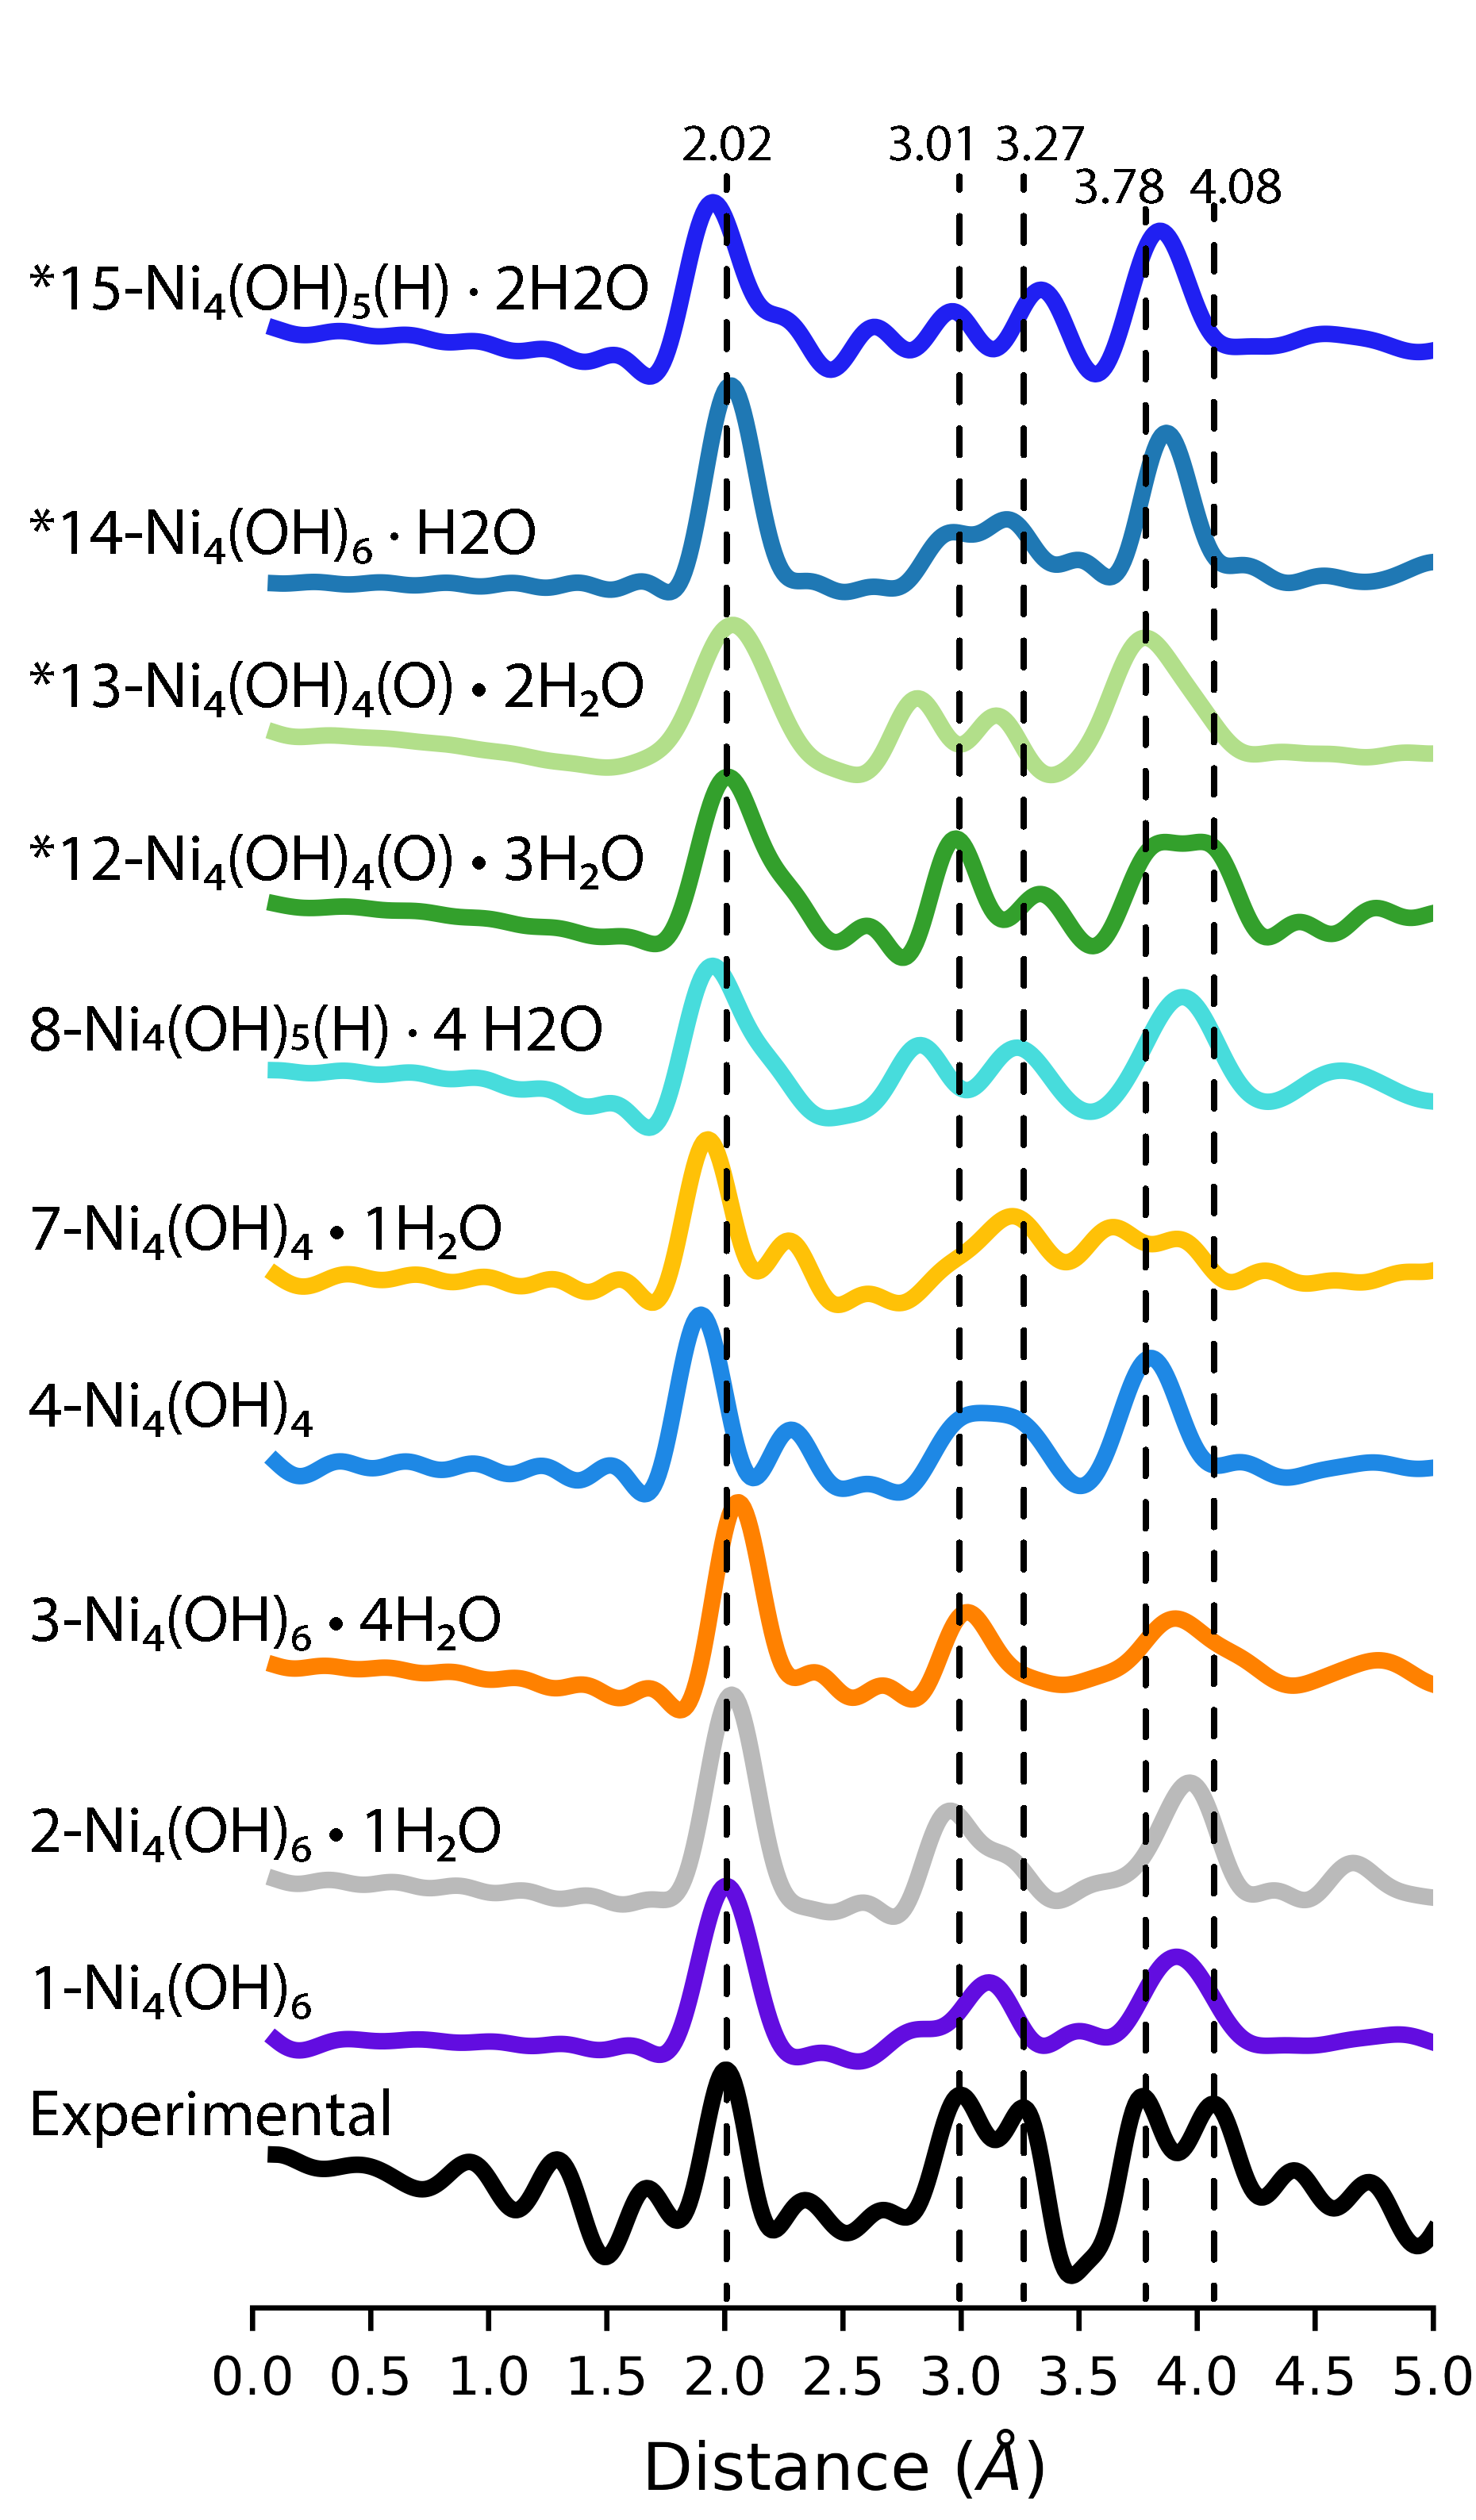
\includegraphics{zi-images/01-Ni-Graphics/2021-04-01-Ni-single-dPDF.png}
    \caption{Differential pair distribution functions (dPDFs) for all the activated structures, using the same color scheme from the \ce{Ni(II)} phase diagram (Figure \ref{fig:phase_diagram_Ni_combined} a)). The dPDFs show the inter-atomic distances between all the atoms of the structure. The key dPDF features seen in the experimental dPDFs \hl{(I should reference back the Platero-Prats article?)} are labeled with dashed lines, with the experimental distances reported underneath in parenthesis. The dPDFs provide a comparison between the experimentally characterized structures and the model structures found from the phase diagram.}
    \label{fig:dPDFs_TandP_trans_Ni}
\end{figure}

We evaluate the performance of our model by comparing the model dPDFs to experimental dPDFs for an activated \ce{Ni} metal complex supported on NU-1000. The synthesized tetranuclear \ce{Ni} cluster exposed to \ce{H2} (3.5\% in \ce{He}) at 200 \degree C for 2 hours and then cooled to 50 \degree C in \ce{H2}.\cite{PlateroPrats2017} Powder X-ray diffraction (XRD) and total scattering data suitable for PDF analysis were collected at 50 \degree C in \ce{H2}.

The dPDFs provide structural insights into the cluster by revealing key interatomic distances with peaks indicating the distance between different atoms. Experimentally, the significant dPDF peaks are the \ce{Ni-O} bond length at 2.02 {\AA}, the \ce{Ni{\Compactcdots}Ni} distances at 3.01 {\AA} and 3.27 {\AA}, and the \ce{Ni{\Compactcdots}Zr} distances at 3.78 {\AA} and 4.08 {\AA}. The experimental, activated dPDFs for \ce{Ni{\Compactcdots}Ni} and \ce{Ni{\Compactcdots}Zr} contain multiple peaks that suggests asymmetric distances within the cluster. \hl{Figure} \ref{fig:dPDFs_TandP_trans_Ni} shows the dPDFs for all the thermodynamically favorable structures found in Figure \ref{fig:phase_diagram_Ni_combined} (a). 


\todo[inline]{Need to update the following section to be more concise (too granular)}
For the \ce{Ni-O} peak, we observe good agreement between the experimental dPDF and the 1-\ce{Ni4(OH)6} (purple) (purple) dPDF. However, the other model structures either under predict (4-\ce{Ni4(OH)4} (light blue), 5-\ce{Ni3(OH)2} (red), and 6-\ce{Ni2(H)2} (lilac)) or slightly over predict (\ce{Ni4(OH)6.41H2O} and 3-\ce{Ni4(OH)6.4H2O} (orange)) the \ce{Ni-O} distance. There is less agreement between the experimental dPDF and the model dPDFs for the \ce{Ni{\Compactcdots}Ni} and \ce{Ni{\Compactcdots}Zr} split peaks. 


None of the model structures recreate the split peaks for \ce{Ni{\Compactcdots}Ni} and \ce{Ni{\Compactcdots}Zr}. 1-\ce{Ni4(OH)6} (purple), \ce{Ni4(OH)4.4H2O} and 4-\ce{Ni4(OH)4} (light blue) show a broad \ce{Ni{\Compactcdots}Ni} peak between 3.01 A and 3.27 A rather than two distinct \ce{Ni{\Compactcdots}Ni} peaks. There is no agreement for 6-\ce{Ni2(H)2} (lilac) and 5-\ce{Ni3(OH)2} (red) compared to the experimental dPDF for the \ce{Ni{\Compactcdots}Ni} peaks, which suggests that the \ce{Ni} composition remains fixed. 



Additionally, 4-\ce{Ni4(OH)4} (light blue) contains a small peak around 2.29 A that is attributed to another \ce{Ni{\Compactcdots}Ni} distance (\hl{see support information}). Again, none of the model structures are able to recreate the split \ce{Ni{\Compactcdots}Zr} split peaks. 1-\ce{Ni4(OH)6} (purple) and 3-\ce{Ni4(OH)6.4H2O} (orange) contain a single peak centered between the two \ce{Ni{\Compactcdots}Zr} split break bounds. 2-\ce{Ni4(OH)6.H2O} (gray) and 4-\ce{Ni4(OH)4} (light blue) also exhibit a single peak; however, this peak is centered around the lower \ce{Ni{\Compactcdots}Zr} split peak bound. For 5-\ce{Ni3(OH)2} (red) and 6-\ce{Ni2(H)2} (lilac), there are no peaks within the \ce{Ni{\Compactcdots}Zr} region. The 5-\ce{Ni3(OH)2} (red) peak at 3.63 A is the \ce{Ni{\Compactcdots}Zr} peak. When transforming with $\ce{H^{*}}$, $\ce{OH^{*}}$, and $\ce{Ni^{*}}$, we observe that the model structures with \ce{Ni} content less than 4 \ce{Ni} per node do not exhibit peak positions that are similar to the experimental dPDF. 

In general, the structures located in Figure \ref{fig:phase_diagram_Ni_combined} (a) are too uncoordinated to match the experimental dPDF. Experimentally, \citeauthor{PlateroPrats2017} found the \ce{Ni} coordination environment be approximately 5.4 under activation conditions.\cite{PlateroPrats2017} The structures shown in Figure \ref{fig:Ni-structure-diagram} fail to match the experimentally observed coordination environment for the \ce{Ni} atoms. Therefore, we explore the stability of the cluster with a fixed \ce{Ni^{*}} composition.

%Despite Figure \ref{fig:structure_diagram_TandP_trans_Ni} suggesting the complete breakdown of the cluster in a bulk-\ce{Ni} species, there is no experimental evidence. Therefore, we remove all structures with a \ce{Ni} compositional less than four and remove the \ce{Ni} transformation in the free energy expression. Figure \ref{fig:phase_diagram_TandP_fixed_Ni} shows the thermodynamic stability as a function of T and P-H2 at a fixed partial pressure of H2O and \ce{Ni} composition. 

The cluster is now transformed with respect to composition of $\ce{H^{*}}$ and $\ce{OH^{*}}$ at a fixed \ce{Ni^{*}} composition (Figure \ref{fig:phase_diagram_Ni_combined} (b)). 1-\ce{Ni4(OH)6} (purple), 2-\ce{Ni4(OH)6.H2O} (gray), 3-\ce{Ni4(OH)6.4H2O} (orange), and 4-\ce{Ni4(OH)4} (light blue) appear on both Figure \ref{fig:phase_diagram_Ni_combined} (a) and (b). The new models appear appearing on \ref{fig:phase_diagram_Ni_combined} (b) are 7-\ce{Ni4(OH)4.H2O} (yellow), 8-\ce{Ni4(OH)5(H).4H2O} (teal), 9-\ce{Ni4(H)2} (mint), 10-\ce{Ni4(OH)2(H)2} (green), and 11-\ce{Ni4(OH)2(H)2.H2O} (pink). These models occupy the phase space of 5-\ce{Ni3(OH)2} (red) and 6-\ce{Ni2(H)2} (lilac) on Figure \ref{fig:phase_diagram_Ni_combined} (a). 

A similar trend is observed in Figure \ref{fig:phase_diagram_Ni_combined} (b) as Figure \ref{fig:phase_diagram_Ni_combined} (a); the continued conversion of \ce{\mu_{2}-OH^{*}} sites into \ce{H2O} with increasing \ce{H2} partial pressure. Starting from 4-\ce{Ni4(OH)4} (light blue), the lowest energy structures exhibit the replacement of \ce{\mu_{2}-OH} ligands with \ce{Ni-H-Ni} structural units. 10-\ce{Ni4(OH)2(H)2} (green) shows the partial conversion of and 9-\ce{Ni4(H)2} (mint) shows the full conversion of the \ce{\mu_{2}-OH} ligands that link the \ce{Ni} atoms of the cluster. Even at low temperatures, adsorbed \ce{H2O} is found in the lowest energy structures (7-\ce{Ni4(OH)4.H2O} (yellow) and 11-\ce{Ni4(OH)2(H)2.H2O} (pink)). 

Interestingly, 8-\ce{Ni4(OH)5(H).4H2O} (teal) exhibits a \ce{Ni-H} and two coordinated \ce{H2O} to the adjacent middle \ce{Ni} atom. However, we also capture a chain of \ce{H2O} molecules that are not coordinated to any of the \ce{Ni} atoms. A structure with these \ce{H2O} removed did not appear to be a thermodynamic minimum after performing \textit{ab initio} thermodynamic analysis. 

% Fixed Ni dPDFs
\begin{figure}[H]
    \centering
    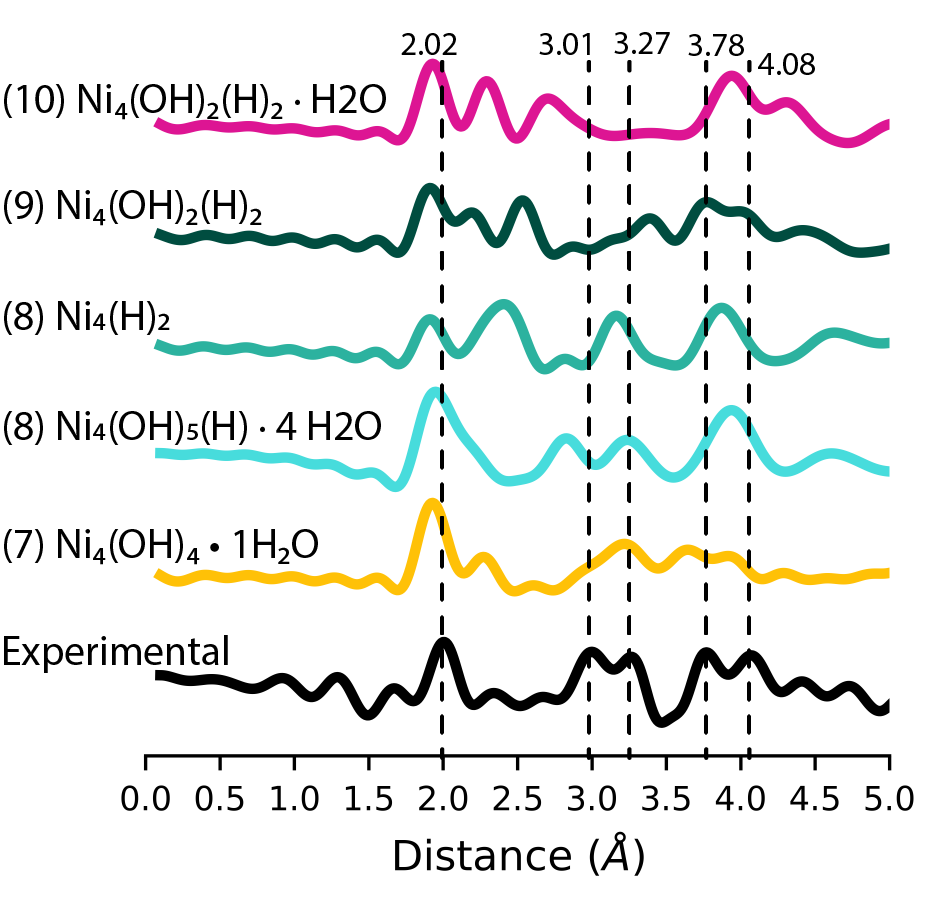
\includegraphics{zi-images/01-Ni-Graphics/2021-03-24-Ni-fixed-dPDFs-manuscript.png}
    \caption{Differential pair distribution functions (dPDFs) for all the activated structures, using the same color scheme from the \ce{Ni(II)} phase diagram (Figure \ref{fig:phase_diagram_Ni_combined} b)). The dPDFs show the inter-atomic distances between all the atoms of the structure. The key dPDF features seen in the experimental dPDFs \hl{(I should reference back the Platero-Prats article?)} are labeled with dashed lines, with the experimental distances reported underneath in parenthesis. The dPDFs provide a comparison between the experimentally characterized structures and the model structures found from the phase diagram.}
    \label{fig:dPDFs_TandP_fixed_Ni}
\end{figure}

We again evaluate the performance of our model system by comparing the model dPDFs to the experimental dPDF by comparing peaks across all structures (Figure \ref{fig:dPDFs_TandP_fixed_Ni}). First, we find that all model structures underpredict the \ce{Ni-O} bond length. Second, we find that as the cluster is reduced and \ce{OH^{*}} are removed a sharp peak appears between 2.1 A and 2.5 A. Inspecting the structures, the peak is related to a \ce{Ni{\Compactcdots}Ni} distance between the two middle atoms of the cluster and is seen by 7-\ce{Ni4(OH)4.H2O}, 9-\ce{Ni4(H)2} (mint), \ce{Ni(NiOH)2(NiH2)}, and 11-\ce{Ni4(OH)2(H)2.H2O} (pink). The split \ce{Ni{\Compactcdots}Ni} peaks are not captured by any of the thermodynamically dominate structures. However, 7-\ce{Ni4(OH)4.H2O} and 9-\ce{Ni4(H)2} (mint) show a single sharp peak centered around the split \ce{Ni{\Compactcdots}Ni} peaks. Interestingly, 11-\ce{Ni4(OH)2(H)2.H2O} (pink) shows no peak within the 3.01 A to 3.27 \AA, but shows a prominent peaks associated to a \ce{Ni{\Compactcdots}Ni} distance at 2.30 {\AA} and 2.71 {\AA}. 9-\ce{Ni4(H)2} (mint) and 11-\ce{Ni4(OH)2(H)2.H2O} (pink) show a single peak within the bounds for the experimental \ce{Ni{\Compactcdots}Zr} split peaks. 10-\ce{Ni4(OH)2(H)2} (green) weakly exhibits the split \ce{Ni{\Compactcdots}Zr} peaks, but includes additional peaks at 2.20 \AA, 2.54 \AA, and 3.40 {\AA} that are attributed to a \ce{Ni{\Compactcdots}Ni} distance. For the \ce{Ni{\Compactcdots}Zr}, 4-\ce{Ni4(OH)4} (light blue) shows a single peak at 3.81 {\AA} and 11-\ce{Ni4(OH)2(H)2.H2O} (pink) shows a single peak at 3.95 {\AA}. 9-\ce{Ni4(H)2} (mint) show a single peak between the experimental peaks at 3.88 \AA, but also features an additional \ce{Ni{\Compactcdots}Zr} peak at 3.17 {\AA}. 10-\ce{Ni4(OH)2(H)2} (green) shows two peaks of unequal height at 3.78 {\AA} and 4.00 {\AA} that are close to the peak positions of the experimental sample. 7-\ce{Ni4(OH)4.H2O} shows \ce{Ni{\Compactcdots}Zr} peak splitting; however, the splitting is shifted to lower positions at 3.66 {\AA} and 3.92 {\AA}. Overall, we observe peak splitting in a few structures, but fail to exactly reproduce the experimental dPDFs from \citeauthor{PlateroPrats2017} 

Interestingly, model 8-\ce{Ni4(OH)5(H).4H2O} (teal) features \ce{Ni-H} and adsorbed \ce{H2O}. For the \ce{Ni-O} peak, 8-\ce{Ni4(OH)5(H).4H2O} (teal) features a broad peak (centered around the 2.02 \AA) is attributed to the range of \ce{Ni-O} distances within the cluster (Figure \ref{fig:atomic-distances-Ni}). Additionally, 8-\ce{Ni4(OH)5(H).4H2O} contains split \ce{Ni{\Compactcdots}Ni} peaks albeit that the split \ce{Ni{\Compactcdots}Ni} peak is shifted to 2.84 {\AA} and 3.25 {\AA} compared to 3.01 {\AA} and 3.27 {\AA}. For the \ce{Ni{\Compactcdots}Zr} split peaks, model 8-\ce{Ni4(OH)5(H).4H2O} (teal) contains a single peak centers between the experimental peaks.   

Again, we find that the bulk of the structures for a fixed \ce{Ni^{*}} under predict the coordination environment for the \ce{Ni} atoms except for the structures at lower \ce{H2} partial pressure and temperature (3-\ce{Ni4(OH)6.4H2O} (orange) and 8-\ce{Ni4(OH)5(H).4H2O} (teal)). This analysis therefore suggests that even during activation conditions \ce{H2O} still is present within the active site structure. We search the model structure library to find structures that more closely match the peak splitting observed experimental and \ce{Ni} coordination environment (Figure \ref{fig:Ni-special-structures}). We find that the following model structures are relevant: 12-\ce{Ni4(OH)4(O).3H2O} (green), 13-\ce{Ni4(OH)4(O).2H2O} (light green), 14-\ce{Ni4(OH)6.H2O} (blue), and 15-\ce{Ni4(OH)5(H).2H2O} (royal). 

\begin{figure}[H]
    \centering
    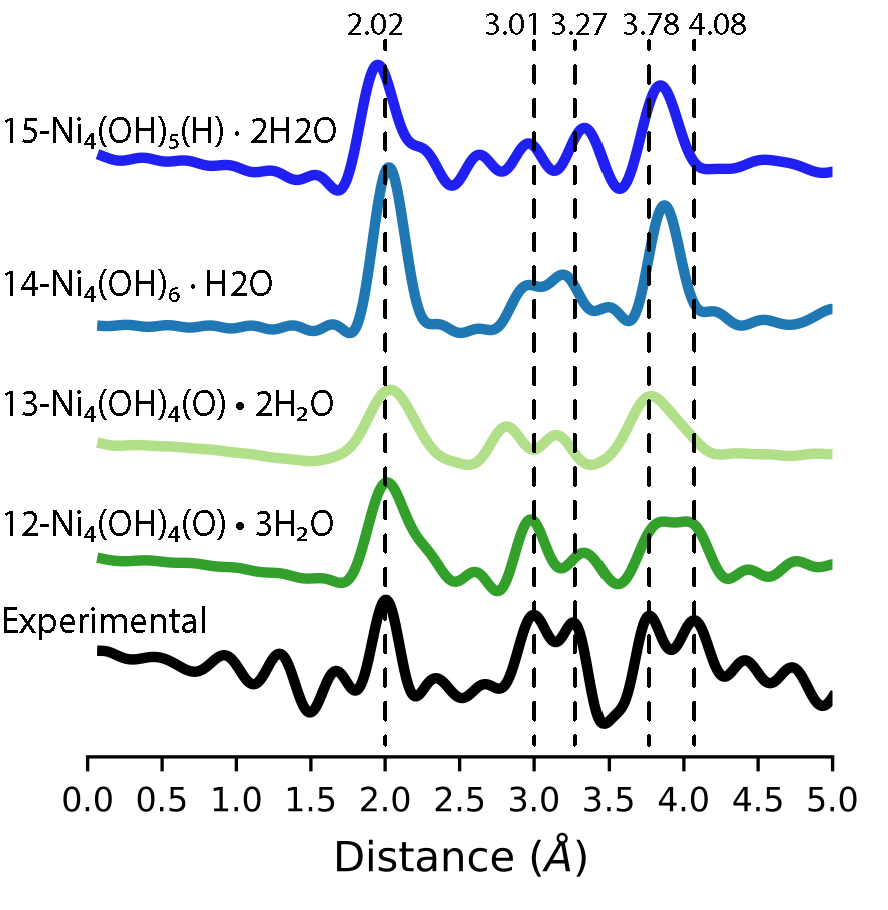
\includegraphics{zi-images/01-Ni-Graphics/2021-03-26-Ni-special-selection-dPDFs-manuscript.png}
    \caption{
    Differential pair distribution functions (dPDFs) for select model structures that do not appear on Figure \ref{fig:phase_diagram_Ni_combined}. The structures shown above are not thermodynamic minimum. The naming convention is adopted: 12-\ce{Ni4(OH)4(O).3H2O} (green), 13-\ce{Ni4(OH)4(O).2H2O} (light green), 14-\ce{Ni4(OH)6.H2O} (blue), and 15-\ce{Ni4(OH)5(H).2H2O} (royal).
    }
    \label{fig:dPDF-Ni-special}
\end{figure}

\begin{figure}[H]
    \centering
    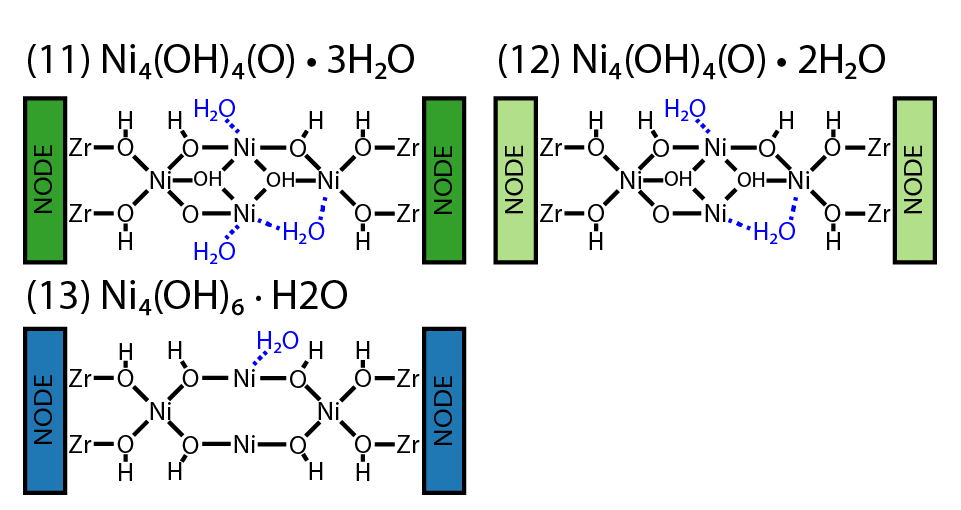
\includegraphics{zi-images/01-Ni-Graphics/2021-figure-structure-Ni-transformations_manuscript-additional-structures.png}
    \caption{
    Schematic representations of the model structures found in Figure \ref{fig:dPDF-Ni-special}, with the following naming convention: 12-\ce{Ni4(OH)4(O).3H2O} (green), 13-\ce{Ni4(OH)4(O).2H2O} (light green), 14-\ce{Ni4(OH)6.H2O} (blue), and 15-\ce{Ni4(OH)5(H).2H2O} (royal). The structures shown here do not represent a thermodynamic minimum from the \textit{ab initio} thermodynamic analysis and therefore do not appear on the phase diagrams. 
    }
    \label{fig:Ni-special-structures}
\end{figure}

Both 12-\ce{Ni4(OH)4(O).3H2O} (green) and \ce{Ni4(OH)4(O).2H2O} (light green) are structurally unique because the cluster proton topology was modified by transforming a \ce{\mu_{2}-OH} ligand to an \ce{\mu_{2}-O} ligand. Although not as pronounced, 12-\ce{Ni4(OH)4(O).3H2O} (green) demonstrates both \ce{Ni{\Compactcdots}Ni} and \ce{Ni{\Compactcdots}Zr} peak splitting. The upper bound for the \ce{Ni{\Compactcdots}Ni} peak is shifted 3.35 A from 3.27 A. The \ce{Ni-O} peak for 12-\ce{Ni4(OH)4(O).3H2O} (green) matches the peak of 2.02 A of the experimental dPDF. However, the \ce{Ni-O} peak for 12-\ce{Ni4(OH)4(O).3H2O} (green) is noticeably broader. The increased width is attributed to the adsorbed \ce{H2O} distance around 2.25 A. 13-\ce{Ni4(OH)4(O).2H2O} (light green) matches the \ce{Ni-O} distance, and does contain split \ce{Ni{\Compactcdots}Ni} peaks that are shifted to lower distances relative to the experimental dPDF. 13-\ce{Ni4(OH)4(O).2H2O} (light green) model does not demonstrate \ce{Ni{\Compactcdots}Zr} peak splitting, but does contain a single peak at the lower \ce{Ni{\Compactcdots}Zr} limit. The 14-\ce{Ni4(OH)6.H2O} (blue) model contains a sharp peak at 2.04 A related to the \ce{Ni-O} distance, \ce{Ni{\Compactcdots}Zr} splitting shifted to lower distances, and a single \ce{Ni{\Compactcdots}Zr } peak within the bounds of \ce{Ni{\Compactcdots}Zr} peak splitting.  The 15-\ce{Ni4(OH)5(H).2H2O} (royal) model structure features split \ce{Ni{\Compactcdots}Ni} peak that closely match the experimental dPDF, but also features another \ce{Ni{\Compactcdots}Ni} peak at 2.64 {\AA} and a broad \ce{Ni-O} peak. The 15-\ce{Ni4(OH)5(H).2H2O} (royal) is the optimized structure of 8-\ce{Ni4(OH)5(H).4H2O} (teal) with 2 \ce{H2O} removed from the structure. The 2.64 {\AA} peak appears with the removal of the \ce{H2O}.

All four structure located on Figure \ref{fig:dPDF-Ni-special} demonstrate matching features to the experimental dPDF, but do not appear on Figure \ref{fig:phase_diagram_Ni_combined} because of their electronic energies. For the same atomic composition, there are structures that are electronically lower in energy. These structures compete with structures at the lower temperatures. 

\begin{figure}[H]
    \centering
    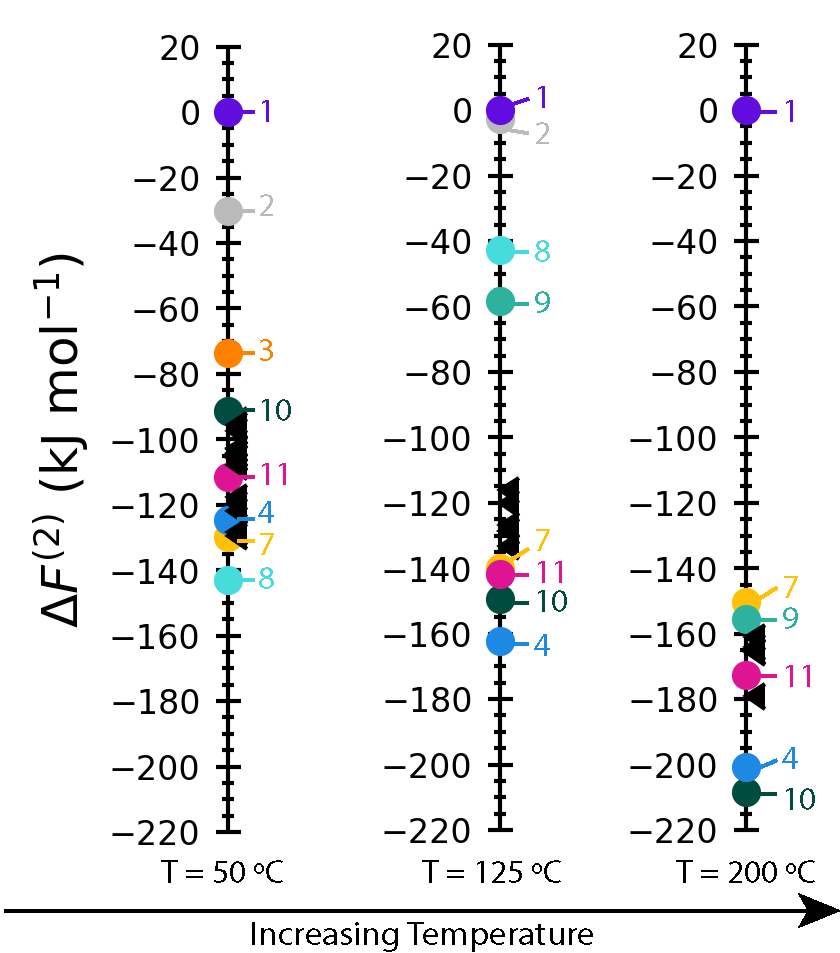
\includegraphics{zi-images/01-Ni-Graphics/2021-figure-lineplot.png}
    \caption{
    The $\Delta F^{(2)}(T,\mu_{\text{H}^{*}},\mu_{\text{OH}^{*}},N_{\text{Ni}^{*}})$ at a fixed \ce{H2} partial pressure of $10^{-5}$ bar and \ce{H2O} partial pressure of $10^{-9}$ bar. As the temperature increases, the thermodynamic landscape within the structure library changes. The colored circles are classified as thermodynamic minimum under some set of conditions, as described by Figure \ref{fig:phase_diagram_Ni_combined}. The colors and numbers are the same previously utilized by Figure \ref{fig:Ni-structure-diagram} and Figure \ref{fig:phase_diagram_Ni_combined}. The black triangles highlight the free energy of a structure within 50 kJ mol$^{-1}$ of the lowest energy structure at the specific set of conditions.
    }
    \label{fig:Ni-relative-energy-plot}
\end{figure}

The phase diagrams, Figure \ref{fig:phase_diagram_Ni_combined}, highlight the most thermodynamically favorable structure at specific conditions. However, the next lowest energy structure is important to consider. We examine the full thermodynamic landscape at a fixed \ce{H2} partial pressure of $10^{-5}$ bar and \ce{H2O} partial pressure of $10^{-9}$ bar while varying the temperature in Figure \ref{fig:Ni-relative-energy-plot}. Additionally, we expand on the thermodynamic minimum in Figure \ref{fig:Ni-relative-energy-plot} to include library structures that are within 50 kJ mol$^{-1}$ of the lowest energy structure at those specific conditions. When considering additional structures within 50 kJ mol$^{-1}$, we determine the significance of the library and the potential for a distribution of active site structures at a specific reaction conditions. The closer in energy the structure is to the lowest energy structure, the more likely the active site is a distribution of active sites rather than the single lowest energy structure. 

%%%%%%%%%%%%%%%%%%%%%%%%%%%%%%%%%%%%%%%%%%%%%%%%%%%%%%%%%%%%%%%%%%%%%
%% Discussion
%%%%%%%%%%%%%%%%%%%%%%%%%%%%%%%%%%%%%%%%%%%%%%%%%%%%%%%%%%%%%%%%%%%%
\newpage
\subsection{Discussion}
%The \ce{Ni(II)} metal complex structure is dependent on the environment. In the absence of any \ce{H2}, the cluster contains four \ce{Ni(II)} atoms interconnected by \ce{OH}-ligands as suggested by \hl{REFERENCE Platero-Prats}. The tetranuclear configuration of the \ce{Ni(II)} cluster spans the c-pore of the NU-1000 framework. When exposed to \ce{H2} gas, the \ce{OH}-ligands provide sites for \ce{H} adsorption onto the cluster resulting in the formation of \ce{H2O}.  \hl{HIGHLIGHT THE SINTERING PAPER} investigate \ce{H2} adsorption and dissociation on a single \ce{Ni} atom also supported on NU-1000, finding that barriers for \ce{H2} adsorption and dissociation and removal of \ce{H2O} are 141 $kJ/mol$. However within our work, we do not look at the kinetics of \ce{H2} adsorption and dissociation and the subsequent removal of \ce{H2O}. Our discussion focuses on the equilibrium thermodynamic structure resulting from exposure to \ce{H2} gas at different partial pressure and temperatures. 


\begin{itemize}
    \item Discussion Topic 1: Comparisons with experiments 
    \begin{itemize}
        \item the conditions that the catalyst experiences, and how those conditions could be different.. and maybe discuss what the goals of those conditions are in terms of the structure of the catalyst
        \item \ce{Ni-H} formation in 8-\ce{Ni4(OH)5(H).4H2O} (teal).. how this structure generates the \ce{Ni-H} that everything thinks is the active species within the catalyst.
        \item 4-\ce{Ni4(OH)4} (light blue) containing the \ce{Ni{\Compactcdots}} peak at 2-ish {\AA}.. dominates the phase space
        \item talk about what these results mean in the context of the activated structure and how the free energies of the structures are very similar in energy.
        \item talk about how, despite the additional \ce{Ni} species, only a single \ce{Ni} atom is the activated metal because structures.. we see that all the other structures are not in good agreement..  
    \end{itemize}
    \item Discussion Topic 2: Formate vs. Formate-Free
    \begin{itemize}
        \item The implications of formate vs. formate-free NU-1000 could impact the structure of the active site, since formate containing blocks potential metal loading sites on the node struture
        \item We model the node structure assuming formate free, but the cluster that is created might actual contain formate species. 
    \end{itemize}
    \item Discussion Topic 3:
    \item Discussion Topic 4:
    
    \item Discussion Topic 1:
    \begin{itemize}
        \item Thermodynamically, active site formation does not demonstrate the formation of a \ce{Ni-H}, which is often to be the active species here. Possible explanation is that the dominate species here is not the \ce{Ni-H}. 
        \item The other explanation is that the \ce{Ni-H} could be the catalytically active site species; however, it might not be the lowest energy structure thermodynamically (meaning that it will not appear in on the phase diagram). There is a possibility that a distribution of active site structures exists, and that the active site structure that is catalytically active is not the dominate structure. 
        \item Additionally, something we did not consider was the \ce{H2} dissociation barriers onto \ce{Ni}. \citeauthor{Li2016sintering} demonstrate a barrier height for the transformation an \ce{OH}-site with \ce{H2} into a \ce{H}-site and \ce{H2O} of around 141 kJ/mol. Having such a high barrier is significant, and does suggest that kinetic limitations could also be present in our model. Our phase diagram is not able to capture, and include these kinetic limitations in the analysis. 
        \item Although we see the breakdown the cluster, kinetic barriers related to \ce{H2} adsorption and dissociation might inhibit the further breakdown of the cluster.
        \item Nonetheless, our model still provides clues into the potential active site structure of the 1-\ce{Ni4(OH)6} (purple) cluster. 
    \end{itemize}
    \item Discussion Topic 2:
    \begin{itemize}
        \item  Comparing the work from \citeauthor{PlateroPrats2017}, the majority of the structures contains under-coordinated \ce{Ni-atoms}. Experimentally, a coordination number of ~5 was observed.
        \item There are features shown on the phase diagram that are not present on the most recent, especially at high \ce{H2} partial pressures. At high \ce{H2} partial pressure, the structures start showing the presence of \ce{Ni-Ni} bonds. The peaks associated with \ce{Ni-Ni} bond formation are not seen experimentally, which suggests the cluster remains largely intact after activation. Throughout our analysis, as the cluster is reduced the formation is \ce{Ni-Ni} bonds is observed.     
        \item The dPDFs are from XRD data that is the average of ALL potential structures within the MOF framework.. the model dPDFs are snapshots of potential structures within the framework here. There is probably a distribution of active site structures that is dominated by the lowest energy structures. 
    \end{itemize}
    \item Discussion Topic 3: Rationalizing some of the experimental mkm work from Hafeera
    \begin{itemize}
        \item Could this help explain some of the discrepancies in reaction trends observed by \citeauthor{Shabbir2020} for \ce{Ni(II)} for \ce{C2H4} hydrogenation? The catalytically active site structure is the \ce{Ni-H} structure. However, thermodynamically, the formation of the \ce{Ni-H} is not dominate. Therefore, only a small number of sites are actually participating in the reaction. \hl{At least for Ni in Hafeera's work this could explain the differences in rates.}
        \item The influence of species such as formate being present on the node. Literature suggests that the reason a cluster forms, and why it forms within the c-pore, is because of the formate ligands capping the \ce{OH/H2O}-ligand pairs of the node. Comparing model and experimental clusters will depend on the experimental synthesis protocols. Only recently was the role of formate understood on the structure of the MOF node.  
    \end{itemize}
\end{itemize}



%\begin{itemize}
%    \item The structural characteristics of the supported metal complexes are dependent on the reaction conditions.
%    \begin{itemize}
%        \item In the presence of a reducing agent (\ce{H2}), the hydroxo-ligands of the supported metal complexes are %removed (as \ce{H2O}). As previously suggested, we show computationally that \ce{H2} is important in breaking the %bonds between the metal clusters and the NU-1000 nodes. We provide the thermodynamic landscape for these %transformations.
%        \item Our findings show similar structural features and suggest that in an \ce{H2} reducing environment these %supported metal complexes containing \ce{OH}-ligands are not stable.  
%        \item At present, our modeling efforts demonstrate the formation of the more mobile \ce{M(0)} species. The breakdown %of the supported metal complex (removal of \ce{OH}-ligands within the cluster) reduces the metal atoms, thereby %generating the mobile \ce{M(0)} species.
%    \end{itemize}
%    \item A key question that still remains is whether these reduced supported metal complexes still exist as a combination %of NPs and multinuclear metal active sites or mononuclear active sites (single-sites) above \SI{200}{Celsius}.
%    \begin{itemize}
%        \item \citeauthor{Halder2020} determined that in an \ce{H2} environment the \ce{Cu3(OH)4} supported metal complexes %showed large \ce{Cu} NP formation. These particles were ~6.0 nm in diameter, which is larger than the ~3.0 nm %diameter hexagonal pore in NU-1000. Therefore, for \ce{Cu}-NU-1000 we know that these NPs grow, and we show using %our modeling that for \ce{Ni} we expect \ce{Ni} NPs to grow as well. 
%        \item Our present results support the experimental findings of \citeauthor{Halder2020} that reduced metal atoms are %generated. However, we extend the findings further and hypothesize that some of the single-site metal atoms remain %intact. Not all of the metal atoms are reduced to \ce{M(0)}; the metal atoms attached to the \ce{OH}-ligands of the %node remain. 
%        \item There are a few more additional calculations to be computed to test our theory (and these calculations are %currently being performed). The calculations contain two single-site models (with and without the \ce{M-H} species). %The metal atoms removed from the system will be accounted for as nanoclusters.
%    \end{itemize}
%\end{itemize}
%We have the following list of questions:
%\begin{itemize}
%    \item Experimentally, there is a different in the protocols to generate the single-site and the clusters in NU-1000? %Experimentally, you can differentiate between the two different catalysts in NU-1000? 
%    \item When looking at the Cu-NU-1000 discussion, did you ever remove the Cu-NPs and determine whether the framework that %was left behind was catalytically active? We wonder whether or not all the metal atoms are becoming the mobile \ce{M(0)} %species. 
%    \item The hexagonal pore returned to its original ~34 A value. How does the value of the pore compare when there are %single-site metal atoms attached to the node? 
%\end{itemize}

\subsection{References}

%The class makes various changes to the way that references are
%handled.  The class loads \textsf{natbib}, and also the
%appropriate bibliography style.  References can be made using
%the normal method; the citation should be placed before any
%punctuation, as the class will move it if using a superscript
%citation style
%\cite{Mena2000,Abernethy2003,Friedman-Hill2003,EuropeanCommission2008}.
%The use of \textsf{natbib} allows the use of the various citation
%commands of that package: \citeauthor{Abernethy2003} have shown
%something, in \citeyear{Cotton1999}, or as given by
%Ref.~\citenum{Mena2000}.  Long lists of authors will be
%automatically truncated in most article formats, but not in
%supplementary information or reviews \cite{Pople2003}. If you
%encounter problems with the citation macros, please check that
%your copy of \textsf{natbib} is up to date. The demonstration
%database file \texttt{achemso-demo.bib} shows how to complete
%entries correctly. Notice that ``\latin{et al.}'' is auto-formatted
%using the \texttt{\textbackslash latin} command.

%Multiple citations to be combined into a list can be %given as
%a single citation.  This uses the \textsf{mciteplus} %package
%\cite{Johnson1972,*Arduengo1992,*Eisenstein2005,*Arduengo%1994}.
%Citations other than the first of the list should be %indicated
%with a star. If the \textsf{mciteplus} package is not %installed,
%the standard bibliography tools will still work but %starred
%references will be ignored. Individual references can be %referred
%to using \texttt{\textbackslash mciteSubRef}:
%``ref.~\mciteSubRef{Eisenstein2005}''.

%The class also handles notes to be added to the bibliography.  These
%should be given in place in the document \bibnote{This is a note.
%The text will be moved the the references section.  The title of the
%section will change to ``Notes and References''.}.  As with
%citations, the text should be placed before punctuation.  A note is
%also generated if a citation has an optional note.  This assumes that
%the whole work has already been cited: odd numbering will result if
%this is not the case \cite[p.~1]{Cotton1999}.

%%%%%%%%%%%%%%%%%%%%%%%%%%%%%%%%%%%%%%%%%%%%%%%%%%%%%%%%%%%%%%%%%%%%%
%% The "Acknowledgement" section can be given in all manuscript
%% classes.  This should be given within the "acknowledgement"
%% environment, which will make the correct section or running title.
%%%%%%%%%%%%%%%%%%%%%%%%%%%%%%%%%%%%%%%%%%%%%%%%%%%%%%%%%%%%%%%%%%%%%
%\begin{acknowledgement}
%
%\hl{authors would like to thank \ldots''.
%
%The author thanks Mats Dahlgren for version one of \textsf{achemso},
%and Donald Arseneau for the code taken from \textsf{cite} to move
%citations after punctuation. Many users have provided feedback on the
%class, which is reflected in all of the different demonstrations
%shown in this document.}
%
%\end{acknowledgement}

%%%%%%%%%%%%%%%%%%%%%%%%%%%%%%%%%%%%%%%%%%%%%%%%%%%%%%%%%%%%%%%%%%%%%
%% The same is true for Supporting Information, which should use the
%% suppinfo environment.
%%%%%%%%%%%%%%%%%%%%%%%%%%%%%%%%%%%%%%%%%%%%%%%%%%%%%%%%%%%%%%%%%%%%%
%\begin{suppinfo}
%
%\hl{This will usually read something like: ``Experimental procedures and
%characterization data for all new compounds. The class will
%automatically add a sentence pointing to the information on-line:}
%
%\end{suppinfo}

%%%%%%%%%%%%%%%%%%%%%%%%%%%%%%%%%%%%%%%%%%%%%%%%%%%%%%%%%%%%%%%%%%%%%
%% The appropriate \bibliography command should be placed here.
%% Notice that the class file automatically sets \bibliographystyle
%% and also names the section correctly.
%%%%%%%%%%%%%%%%%%%%%%%%%%%%%%%%%%%%%%%%%%%%%%%%%%%%%%%%%%%%%%%%%%%%%
\newpage
\bibliography{achemso-demo}

\end{document}